%%%%%%%%%%%%%%%%%%%%%%%%%%%%%%%%%%%%%%%%%%%%%%%%%%%%%%%%%%%%%%%%%%%%%%%%%%%%%%%%
\documentclass[letterpaper, 10 pt, conference]{ieeeconf}  


\IEEEoverridecommandlockouts                              % This command is only needed if 
% you want to use the \thanks command

\overrideIEEEmargins                                      % Needed to meet printer requirements.

% See the \addtolength command later in the file to balance the column lengths
% on the last page of the document

%======== Packages ========%
% The following packages can be found on http:\\www.ctan.org
\usepackage{amsmath}
\usepackage{amsfonts}
\usepackage{amssymb}
\usepackage{graphicx}
\usepackage{subcaption}
\usepackage{indentfirst}
\usepackage{algpseudocode}
\usepackage{algorithm}
\usepackage{cite}
\usepackage[capitalize]{cleveref}
\usepackage{comment}

%======== Todonotes ========%
\usepackage{todonotes}
\usepackage{soul}
\usepackage{gensymb} % for the use of \degree that shows degree symbol
\definecolor{smoothgreen}{rgb}{0.7,1,0.7}
\sethlcolor{smoothgreen}

\newcommand{\todopara}[1]{\vspace{0px} %
	\todo[inline, color=black!10]{\textbf{[Paragraph:]} {#1}} %
}
\newcommand{\todonote}[1]{\vspace{0px} %
	\todo[inline, color=green!30]{\textbf{[Note:]} {#1}} %
}
\newcommand{\todoQ}[1]{\vspace{0px} %
	\todo[inline, color=orange!50]{\textbf{[Note:]} {#1}} %
}
\newcommand{\todohere}[1]{\hl{(\textbf{TODO:} #1)}}

\newcommand{\hidetodos}{
	\renewcommand{\todopara}[1]{}
	\renewcommand{\todonote}[1]{}
	\renewcommand{\todoQ}[1]{}
	\renewcommand{\todohere}[1]{}}

%======== Titles and Authors ========%
\title{\LARGE \bf
	Interacting multiple model-based human motion prediction for motion planning of companion robots*
}

\author{Donghan Lee$^{1}$, Chang Liu$^{2}$ and J. Karl Hedrick$^{3}$% <-this % stops a space
	\thanks{*This work was not supported by any organization}% <-this % stops a space
	\thanks{$^{1}$Donghan Lee with the Vehicle Dynamics \& Control Lab, Department of Mechanical Engineering, University of California at Berkeley, California 94720, USA
		{\tt\small donghan.lee@berkeley.edu}}%
	\thanks{$^{2}$Chang Liu with the Vehicle Dynamics \& Control Lab, Department of Mechanical Engineering, University of California at Berkeley, California 94720, USA
		{\tt\small changliu@berkeley.edu}}%
	\thanks{$^{3}$J. Karl Hedrick is with Faculty of Mechanical Engineering, University of California at Berkeley, California 94720, USA
		{\tt\small khedrick@berkeley.edu}}%
}

%======== Paper Content ========%

\begin{document}
	
	\maketitle
	\thispagestyle{empty}
	\pagestyle{empty}
	
	%%%%%%%%%%%%%%%%%%%%%%%%%%%%%%%%%%%%%%%%%%%%%%%%%%%%%%%%%%%%%%%%%%%%%%%%%%%%%%%%
	\begin{abstract}
		Motion planning of human-companion robots is a challenging problem and its solution has numerous applications. 
		This paper proposes a motion planning method for human-companion robots to accompany humans in a socially desirable manner, which takes into account the safety, comfortableness and naturalness requirements.
		A unified Interacting Multiple Model (IMM) framework is developed to estimate human motion states from noisy sensor data and predict human positions in a finite horizon.
		The robot motion planning is formulated as a model predictive control problem to generate socially desirable motion behavior based on the predicted human positions.
		% The proposed approach generates an accompanying behavior that takes into account the safety, comfortableness and naturalness requirements.
		% Such IMM-based estimation and prediction framework incorporates different dynamic models and computes mode probabilities of each model, which is suitable for human motion prediction as human motion usually involves different patterns.
		% To deal with the nonlinear dynamics of the human motion, Unscented Kalman filter (UKF) is applied to each model in the IMM framework.
		The effectiveness of the proposed motion planning method in facilitating the socially desirable companion behavior is evaluated through simulations and the advantage of IMM framework for human motion estimation and prediction compared to traditional single-model approaches has been demonstrated.
	\end{abstract}
	
	%%%%%%%%%%%%%%%%%%%%%%%%%%%%%%%%%%%%%%%%%%%%%%%%%%%%%%%%%%%%%%%%%%%%%%%%%%%%%%%%
	
	\section{INTRODUCTION} \label{sec:intro}
	The application of autonomous robots for search-and-rescue (SAR) missions have received considerable attentions in last decades \cite{,,}.
	One particular interesting scenario is allowing autonomous robots to accompany humans during the SAR.
	Robot companions can follow and assist humans in carrying heavy apparatus, exploring dangerous areas or detecting signals of survivors.
	% Motion planning of human-companion robots is a challenging problem and its solution has numerous applications, such as for accompanying elderlies at home and guiding visitors in museums. 
	
	Socially desirable companion behavior necessitates several requirements to be satisfied, including safety, comfort, naturalness and sociability \cite{kruse2013human}.
	Among these requirements, safety serves as the fundamental guideline, requiring that robots avoid collision with accompanied humans under all circumstances \cite{hoeller2007accompanying,fox1997dynamic,svenstrup2010trajectory}.
	% 	\todohere{use lit from the survey paper. explain many aspects of social navigation. However, in problem formulation, just list what is done in this paper: focus on comfortableness (distance using proxemics and velocity similarity)}
	Comfort composes a social requirement on the robot behavior, which requires robots to pose little annoyance and stress for the accompanied humans \cite{kruse2013human}.
	It is mainly formulated regarding the distance that a robot needs to keep from people.
	For example, Hall \cite{hall1968proxemics} proposed the concept of ''Proxemics" to denote the virtual zone around a person that other people should avoiding entering in order to prevent the discomfort the person may feel.
	Barnaud et al.\cite{barnaud2014proxemics} investigated the proxemics models in the context of human-aware robot navigation by investigating a classic corridor-crossing experiment.
	This work provides a tool for designing parameters of the proxmics model that can be used for robot motion planning in the environment with human existence.
	Naturalness and sociability reflect the requirements on \todohere{finish this sentence}.
	%     \todohere{rephrase the following sentence:}
	%     In \cite{takayama2009influences}, authors extract robot design principles for approaching distance and gaze depending on social context.
	
	\todohere{move the following sentence to the method review section}
	By incorporating these requirements into account, researchers have developed several human-companion robots. 
	In \cite{kirby Companion: A constraintoptimizing method for person acceptable navigation}, a generalized framework for representing social conventions as components of a constrained optimization problem was presented and it was used for path planning and navigation.
	
	% the former requires robots to maintain appropriate distance from humans and the latter emphasizes on the similarity in motion speeds between robots and humans. 
	% This requires robots to stay within a proper distance from the accompanied person while avoiding collision with him/her.
	% In fact, aside from the traditional requirement of robot path planning that focuses on obtaining the optimal path from one position to another in real-time, the human-aware robot motion planning needs to take the existence of humans into account.
	% This imposes certain requirements on the robot motion, such as safety, comfortableness and naturalness.
	% Safety serves as the fundamental requirements for robots to interact with humans and it requires robots to avoid hurting humans. 
	% Based on the definition in \cite{kruse2013human}, comfortableness requires robots to pose little annoyance and stress for humans and naturalness emphasizes the similarity between robots and humans in low-level behavior patterns.
	% In this work, we develop an approach for robots to follow humans in real time without the prior knowledge of the human trajectory. 
	% The planned robot motion takes the safety, comfortableness and naturalness requirements into consideration.
	
	Cosgun et al.\cite{cosgun2013autonomous} develops a robot for telepresence usage, which uses the laser scanner to track human movement and predicts human path by extrapolating based on the estimated human position and speed, assuming a constant velocity human motion model.
	The robot utilizes the depth-limited breadth-first search approach to find the waypoints around the predicted human positions so that the robot can always face the accompanied human with a similar velocity as the human.
	Hoeller et al.\cite{hoeller2007accompanying} presents a local path planning approach for the companion robot to stay in proximity to the target person and simultaneously prevent colliding with any passers-by. 
	The probabilistic roadmaps is used to plan collision-free paths to a given target location, chosen based on the predicted adjacent humans' positions.
	A laser-based people tracking technique is used to estimate the motions of humans and a potential field method is applied for predicting the humans’ future trajectories.
	
	%	Artificial Neural Network (ANN) is adopted for human motion prediction. 
	To generate socially desirable motion behavior, accurate human motion estimation and prediction is necessary, which can be then utilized for robot motion planning.
	% We divide the human-accompanying motion planning into three steps.
	To be specific, a robot needs to estimate motion states of the accompanied human in real time based on measurements from equipments such as GPS sensors or cameras and then predict human future trajectory.
	% Due to the sensor noise, measurement results need filtering.
	There exist several widely-adopted estimation methods, such as the Kalman filter\cite{welch1995introduction}, which provides the minimum mean square error estimation of states for linear systems with Gaussian noise. \todohere{find references for its application to motion estimation and prediction}
	The Extended Kalman filter (EKF) and Unscented Kalman filter (UKF) \cite {KalmanFiltering}, which are extensions of the KF for nonlinear systems, have also been applied for motion estimation and prediction\cite{key}. 
	EKF can be obtained by applying the KF to the first-order Taylor expansion of nonlinear systems while UKF uses a deterministic sampling technique, called the Unscented Transform, to perform a stochastic linearization through the use of a weighted statistical linear regression process \cite{thrun2005probabilistic}.
	\todohere{if the references for motion estimation and prediction using xKF methods can be found, then remove the following part.}
	Based on the estimated states, extrapolation assuming known human motion models, such as the constant velocity and constant turn model \todohere{lit review}, can be applied for predicting human positions in a finite horizon.
	\todonote{try to merge the following sentence with the previous one. }
	These methods usually assumes a single motion model for estimation and prediction and have been widely applied in motion planning and localization in the field of robotics \cite{thrun2005probabilistic}.
	
	In recent years, machine learning techniques have been utilized for human motion prediction.
	% 	In \cite{wu2012path}, Wu et al. developed a path prediction approach by back propagating through a trained Netural Network. 
	%     The proposed method is shown to be able to predict abrupt human direction change when a person makes turns. 
	Bennewitz et al. \cite{bennewitz2005learning} proposed a technique for learning collections of trajectories that characterize typical motion patterns of persons
	Trajectories were clustered using Expectation Maximization algorithm and a hidden Markov model was then applied to predict future positions of persons based on sensory input in real time.
	Fulgenzi et al. \cite{fulgenzi2008probabilistic} developed an approach for predicting trajectories of moving objects, which were supposed
	to move with typical patterns with some amount of uncertainty. 
	Those patterns were represented by Gaussian processes and pre-learned based on the collected set of trajectories.
	A two-layer prediction that combined long-term destination inference and short-term motion prediction was proposed in \cite{foka2010probabilistic}:
	the short-term prediction that refers to the one-step ahead prediction of a human’s future position was achieved by a Polynomial Neural Network (PNN), which was trained offline;
	the long-term prediction was performed by utilizing the heading direction of a human to determine the destinations where he/she would have interest in visiting.
	%     These locations were pre-defined by utilizing the human motion data.
	%     Ziebart et al. \cite{ziebart2009planning} proposed the maximum entropy inverse optimal control approach for modeling goal-directed trajectories of pedestrians.
	%     Such modeling method offers the benefit of the generality of its learned cost function to changes in the environment and to entirely different environments.
	% 	\todohere{more references on human motion estimation and prediction.}
	
	These approaches have achieved success in predicting human motion trajectories.
	However, they usually involves the collection of training data (e.g., recorded human trajectory) and are prone to be scenario specific. 
	In fact, human motion can be well predicted using these machine learning-based prediction approaches in the scenarios where human trajectories have been collected used for training predictors.
	However, these predictors may fail to obtain accurate prediction in unknown environments.
	This drawback renders the machine learning-based methods less applicable for search and rescue missions since disaster sites are rarely similar to the known ones and therefore robots need to work in unfamiliar environments.
	
	Human motion usually involves different identified motion models, such as straight-line movement, making turns and change of speed.
	Therefore, a model-based approach would be promising to generate accurate prediction results.
	In this work, we employ the Interacting Multiple Model (IMM) approach for human motion estimation and prediction.
	IMM is a model-based estimation framework that takes into several system models into account and dynamically adjusts the mode probabilities. 
	To deal with the nonlinear dynamics of the human motion (such as making turns), UKF is applied to each model in the IMM framework, resulting in the so-called IMM-UKF approach.
	Such approach can achieve higher accuracy compared to traditional estimation and prediction methods that utilize a single motion model. 
	Additionally, no training is needed and thus scenario-independent, which is advantageous over machine learning methods for search and rescue missions.
	Utilizing the predicted human trajectory, a model predictive control (MPC)-based motion planner is developed for the companion robot to autonomously accompany the target person in a socially desirable manner, which takes into consideration the safety and comfort requirements.
	The main contribution of this paper is ... \todohere{need to fill this paragraph}.
	% 	The proposed motion planning method differs from previous works in several aspects.
	% 	First, different from the single-model based estimation and prediction approaches used in \cite{cosgun2013autonomous,hoeller2007accompanying}, the IMM-UKF method incorporates different human movement models into account, which results in higher estimation and prediction accuracy, especially when humans motion involves complex patterns.
	% \cite{cosgun2013autonomous,hoeller2007accompanying} does not deal with.
	% 	Second, the model-based IMM-UKF approach does not require training data and is scenario-independent, which is advantageous over the machine learning methods, such as the ANN method in \cite{bennewitz2005learning,fulgenzi2008probabilistic,foka2010probabilistic}. 
	% 	\todohere{emphasize on the benefit of MPC}
	% 	Additionally, MPC-based planner recursively solves a nonlinear program for the optimal trajectory over finite horizon. 
	% 	Motion requirements such as the safety and comfort can be easily incorporated in the objective function and constraints of the nonlinear program.
	% 	\todonote{need to find more ref about motion planning methods for navigating in human environments}
	% 	Besides, such MPC-based planner can be implemented in real-time, which makes it suitable for dynamic environments. 
	%     This differs from some sampling-based planning methods, such as that requires large computation time potential field based methods, such as in \cite{hoeller2007accompanying}, which needs careful design of potential functions to enforce all these requirements.
	%Our approach provides a general and efficient way for autonomous robots to accompany humans. 
	
	%	By using the predicted human positions in the prediction horizon, the robot motion planning is formulated as an MPC problem that explicitly considers safety, comfortableness and naturalness requirements on the robot motion behavior. 
	% The motion prediction composes an interesting but difficult topic due to the lack of a precise human dynamics model. 
	% Several methods have been utilized such as regression-based approaches\cite{trautman2012probabilistic} and learning-based approaches\cite{vasquez2014inverse,wu2012path}.
	%In this work, we employ the estimated human states from the IMM estimator and extrapolate them for predicting human future states.
	
	%The second part of the motion planner requires a time-efficient motion planning method that can generate motion behavior in accordance with the aforementioned safety, comfortableness and naturalness requirements.
	% refers to the robot motion planning based on the predicted human states.
	% Motion planning considering constraints, such as the aforementioned safety, comfortableness and naturalness requirements, tends to be difficult.
	%	Time-efficient motion planning approaches that generate socially desirable trajectory is desirable.
	%	Various planning algorithms, such as the potential field method\cite{khatib1986real} \todohere{explain more details} and the graph-search-based techniques\cite{cosgun2013autonomous} \todohere{explain more details} have been developed and successfully applied.
	%	However they usually assume simple kinematic model of robots and cannot take into account complex constraints, which renders these methods less suitable for human-companion motion planning in a socially desirable manner.
	% We adopt the model predictive control (MPC) approach that can explicitly model and compute the desired robot behavior.
	
	The remainder of this paper is organized as follows:
	first, the problem of motion planning for a human-companion robot is formulated for the SAR mission;
	second, the IMM-UKF estimation and prediction method is described, followed by the MPC planner;
	%\cref{sec:simulation} presents the simulation setup for evaluating the method, followed by results and discussions in \cref{sec:results}. 
	next, simulation setup and results on evaluating the proposed approach are presented; 
	lastly, concluding remarks and ideas of future work are presented.
	
	
	%\begin{figure}
	%\centering
	%\includegraphics[width=0.31\textwidth]{figures/field_3}
	%\caption{Illustration of the field of interest}\label{fig:field}
	%\end{figure}
	
	\section{PROBLEM FORMULATION}\label{sec:formulation}
	Considering the SAR scenario (\cref{fig:ref_traj_init}) in which a human first responder needs to deliver medical treatment to several destinations that contain injured people. 
	A companion robot that carries medical apparatus will accompany the human and sequentially move to these destinations.
	The human follows the trajectory that is shown in \cref{fig:ref_traj_end}.
	Such trajectory covers several typical human motion patterns, including straight-line movement, motion following curved paths and making sharp turns.
	% The red circle and the green triangle at the lower-left corner denote the human and the robot, respectively. 
	The robot has no knowledge about the positions of human destinations, nor the pre-designed human trajectory.
	However, it can measure human positions in real time from the GPS sensor that the human carries.
	Several obstacles exist in the field, including five stationary ones and two moving ones, representing unmovable obstructions, such as buildings or plants, and mobile objects, such as pedestrians or vehicles, respectively.
	\cref{fig:ref_traj_obs1,fig:ref_traj_obs2} show that the moving obstacles start to act.
	The positions of stationary obstacles are known to both the human and the companion robot while the moving obstacles are measured using same measurement tool for tracking the human rescuer.
	%	Neither the human nor the robot can step into or cross these obstacles. 
	When accompanying the human, the robot should satisfy the aforementioned safety and comfort requirements.
	%     , which requires the robot to avoid colliding with either the human or any obstacles and maintain a proper distance from the accompanied human.
	To be specific, a circular “safety zone" with radius $d_s$ (\cref{fig:safe_zone}) is defined around the target person, indicating the area that the robot should avoid entering.
	Stepping into the "safety zone" is considered as unsafe behavior and thus should be avoided.
	The comfort requirement consists of two parts: the robot needs to maintain a comfortable distance $d_c$ from the human, as investigated in \cite{hall1968proxemics}, and also keep similar speed with the human, as shown in \cite{ref}.
	
	%We apply our method to the robot so that it can track the human motion and plan its own behavior.
	%The performance of the robot will be evaluated based on these three requirements.
	
	\begin{figure}
		\centering
		\begin{subfigure}{0.2\textwidth}
			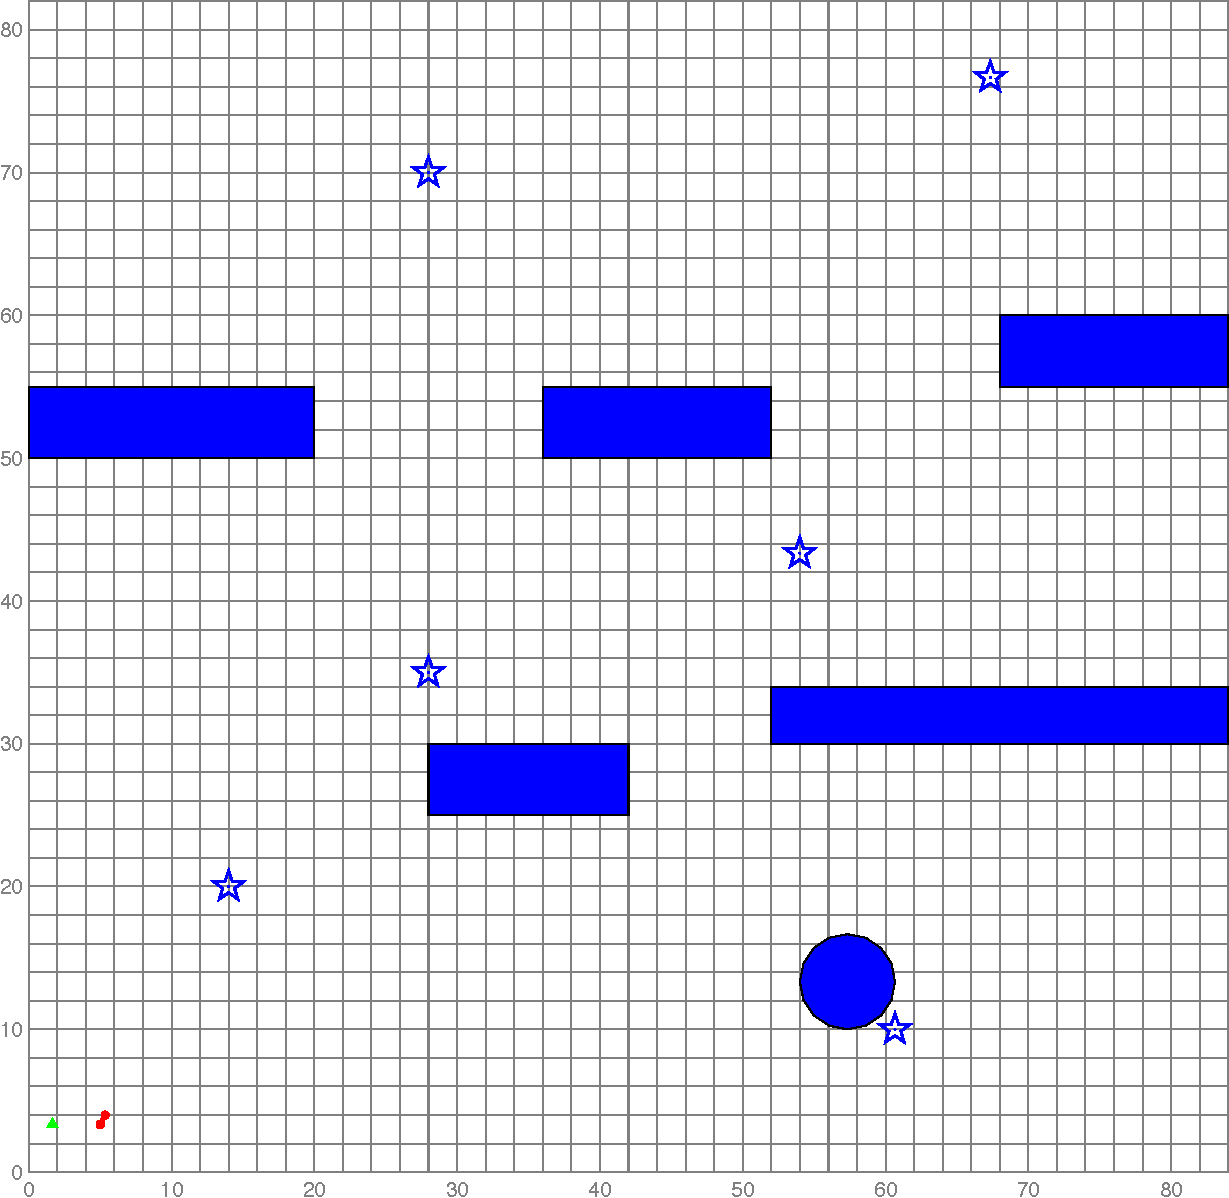
\includegraphics[width=\textwidth]{figures/ref_traj_init}
			\caption{}
			\label{fig:ref_traj_init}
		\end{subfigure}
		~
		\begin{subfigure}{0.2\textwidth}
			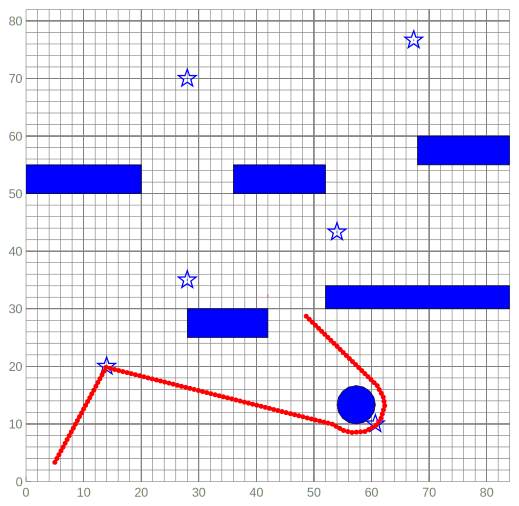
\includegraphics[width=\textwidth]{figures/ref_traj_obs1}
			\caption{}
			\label{fig:ref_traj_obs1}
		\end{subfigure}
		~
		\begin{subfigure}{0.2\textwidth}
			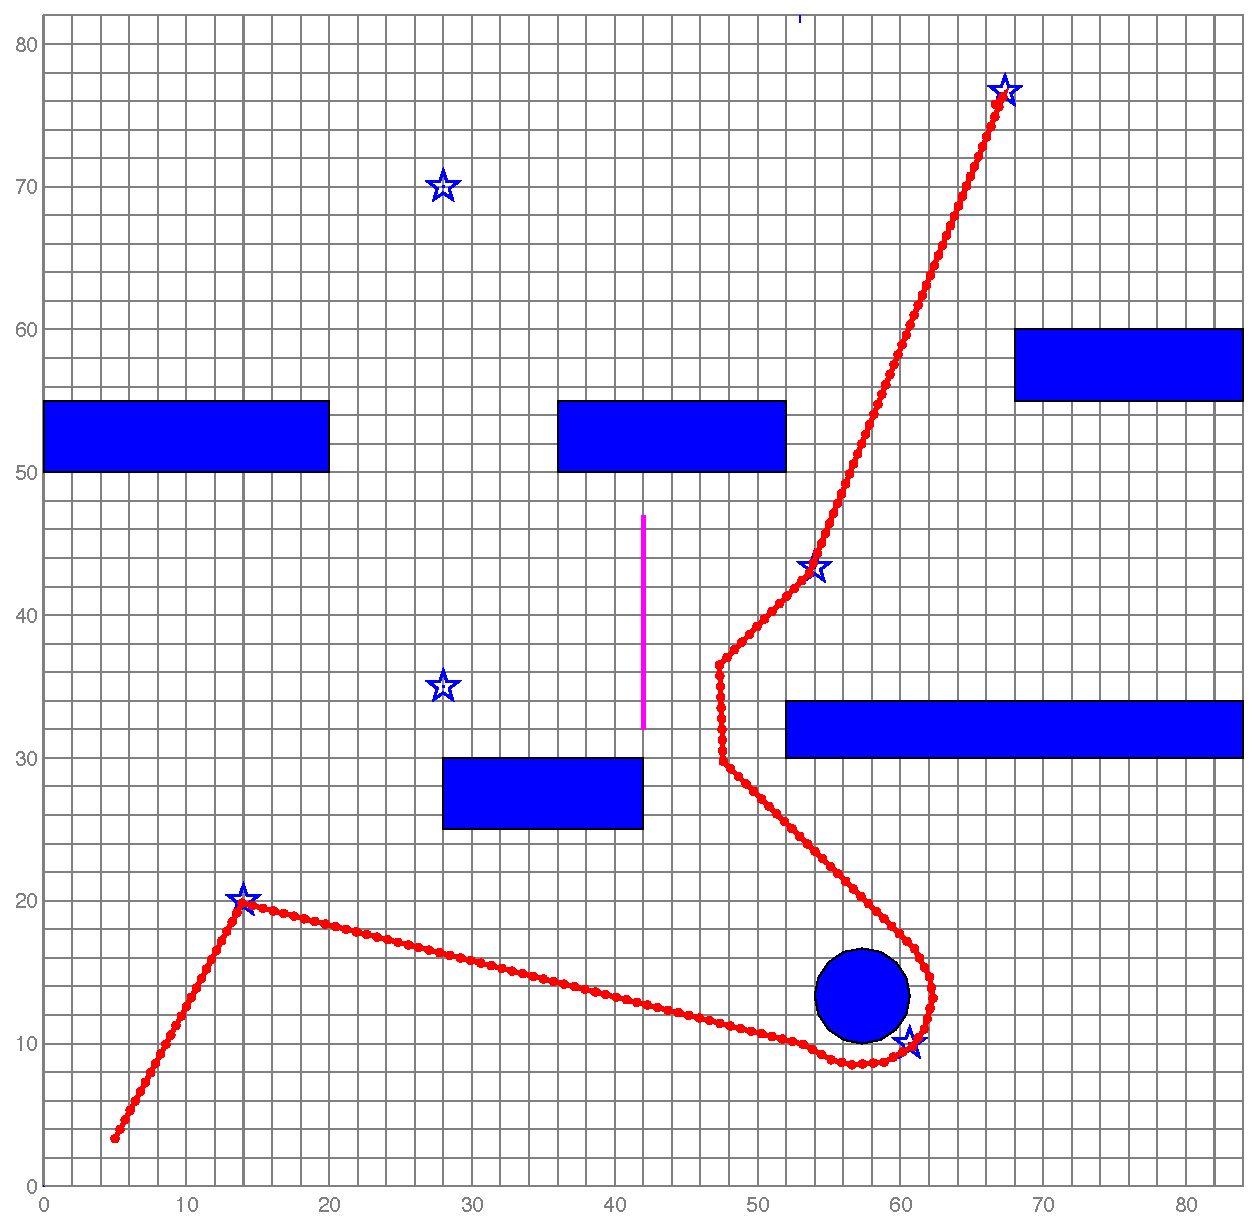
\includegraphics[width=\textwidth]{figures/ref_traj_obs2}
			\caption{}
			\label{fig:ref_traj_obs2}
		\end{subfigure}
		~
		\begin{subfigure}{0.2\textwidth}
			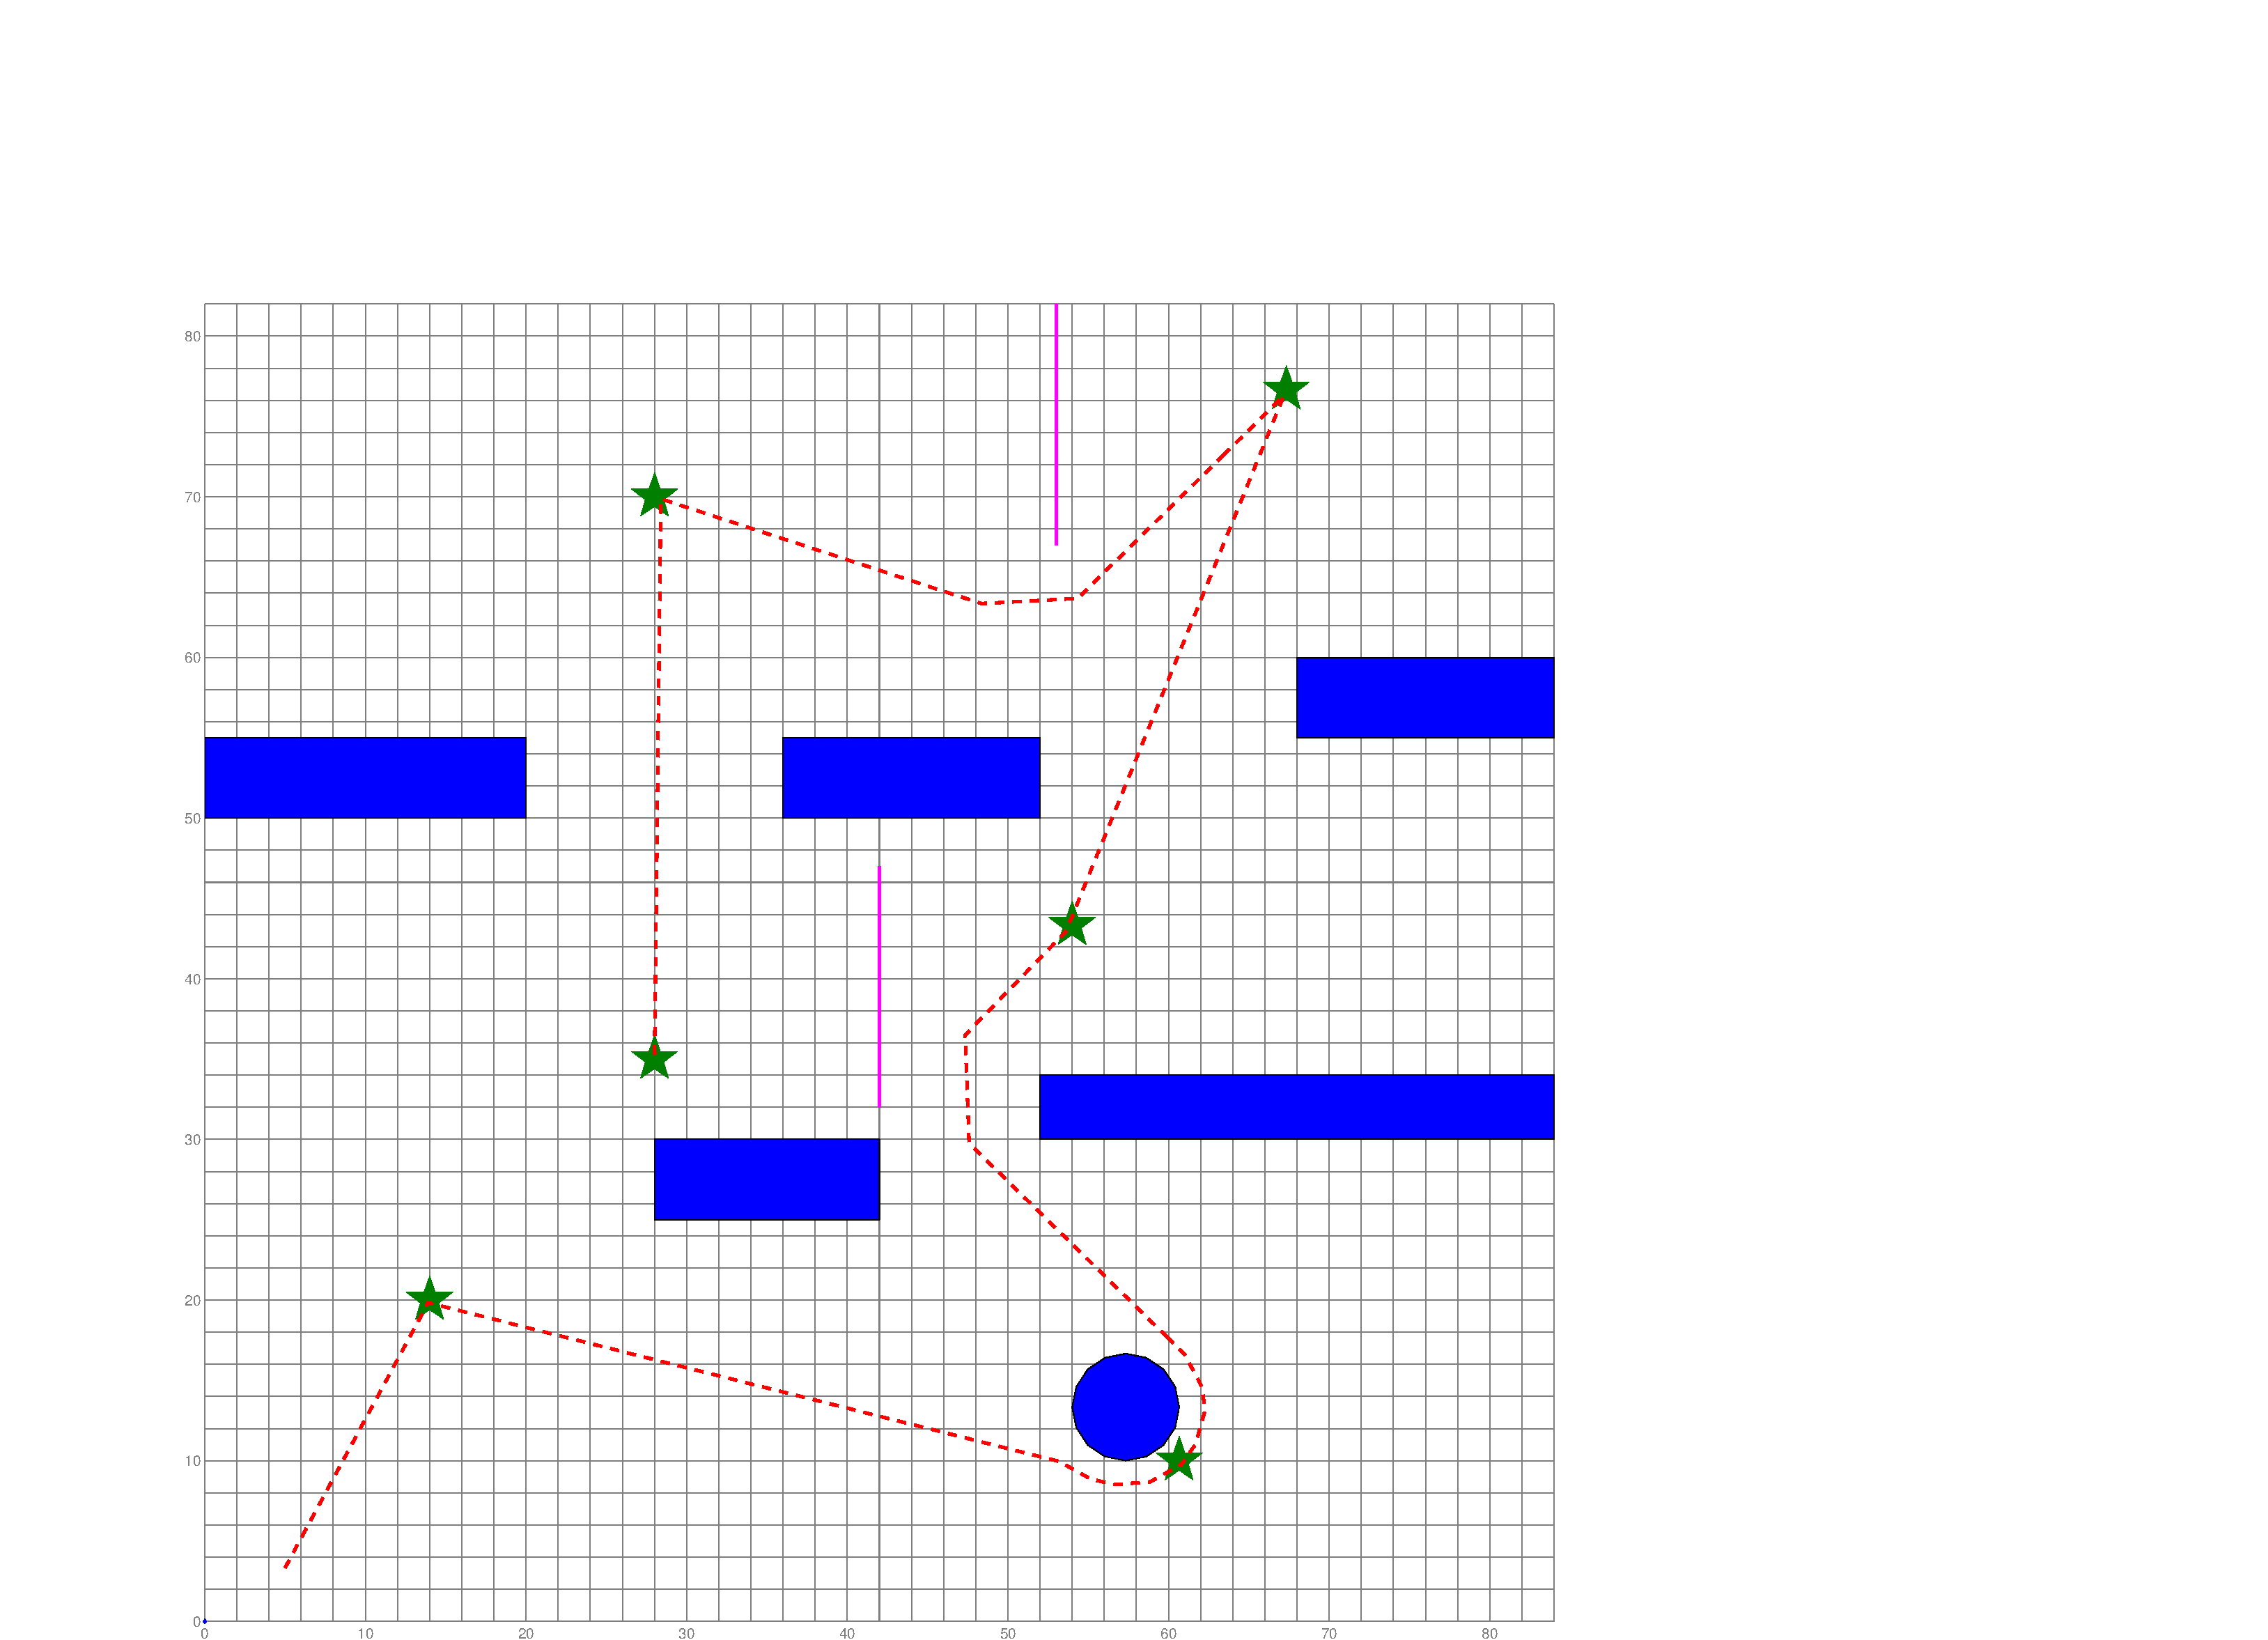
\includegraphics[width=\textwidth]{figures/ref_traj_end}
			\caption{}
			\label{fig:ref_traj_end}
		\end{subfigure}
		\caption{A search-and-rescue scenario for the companion robot to accompany a human. (a) The initial state of the scenario. The red circle and the green triangle represent the human rescuer and the robot companion, respectively. Stars denote human destinations and the blue rectangles stand for static obstacles. (b) The $1^\text{st}$ moving obstacle starts moving. (c) The $2^\text{nd}$ moving obstacle starts moving. (d) The full human trajectory.} \todonote{dh: change moving obstacles' color to make it more obvious; add arrows to them to show the direction. }
	\end{figure}
	
	
	\section{METHODS} \label{sec:framework}
	%Effective human-accompanying requires the robot to perform three steps: human tracking, human motion prediction and robot motion planning.
	%First, the robot needs to estimate human states over time from noisy sensor data.
	%Second, the robot needs to predict human motion in the future based on the estimation results.
	%Based on the prediction, the robot plans its own motion in a socially acceptable way.
	%The following subsections details the methods for each of the three steps.
	
	\subsection{Human Motion Estimation}\label{subsec:human_track}
	The Interacting Multiple Model (IMM) approach are applied for estimating the human motion from the noisy sensor data.
	% 	The IMM approach has been generally considered as the mainstream method for maneuvering target estimation. 
	It utilizes a bank of $r$ number of filters, each (designed to model) \todohere{corresponding to} a different dynamics.
	% IMM algorithm is a sub-optimal algorithm based on the minimum mean square error criterion. 
	%	State estimate at time $k$ is computed with mode probabilities and state estimates from each possible current model associated with one of the $r$ filters, using the following formula:
	State estimate at time $k$ is computed as a weighted sum of estimates from each filter, as shown in the following formula:
	\todoQ{$mu_i$ or $mu_j$?}
	\[
	\hat{x}(k|k)=\sum\limits_{j=1}^{r}\mu_j(k)\hat{x}^j(k|k)
	\]
	where $r$ denotes the number of models; $\hat{x}^j(k|k)$ represents the state estimate from the $j^\text{th}$ filter; $\mu_j(k)$ stands for the mode probability and is computed as follows:
	\[
	\mu_j(k)=\frac{1}{c}\sum\limits_{i=1}^{r}L_{ij}(k)p_{ij}\mu_j(k-1)
	\]
	where $c$ denotes the normalizing factor; $L_{ij}(k)$ stands for the likelihood function and $p_{ij}$ represents the mode transition probability from the $i^\text{th}$ to the $j^\text{th}$ model. 
	Each filter uses the mixed initial state estimate and covariance from different combination of the previous model. 
	Readers interested in the details of the IMM approach can refer to \cite{yaakov2002estimation}.
	% 	The IMM approach offers the benefits of incorporating multiple motion models in the estimation process, which makes it suitable for human state estimation since when a person moves, it usually involves multiple motion patterns.
	% We now motivate the use if nonlinear models in the IMM by introducing a popular nonlinear model used in target tracking. It is the Coordinated Turn model, whose name is derived from the aerospace industry. A coordinated turn is a turn in which the turn rate and speed are constant. If the turn rate is a known constant the model is linear. \cite {derek_phd_dissertation} 
	
	% Unfortunately, the turn rate of the human is rarely constant. Thus the coordinated turn model will be augmented with the turn rate as additional state. Therefore it is necessary to use an nonlinear system.
	In this work, two different dynamic models are used in the IMM framework: one is the coordinated turn motion model, reflecting the action of making turns or moving along a curved path, and the other is the uniform motion model, representing the straight-line movement. 
	The equation of motion for the both the coordinated turn motion and uniform motion model becomes the following \todohere{is this the equation of turn motion model only?}
	\begin{subequations}
		\begin{align}
			x^{h,1}(k+1)&= f(x^{h,1}(k))+Gw(k)\\
			%Q(k)&=E[w(k)w(k)^\top]
			f(x^{h,1}(k))&=\left[
			\begin{array}{c}
				p^h_1+\frac{\sin(\omega^h T)}{\omega^h}v^h_1-\frac{1-\cos(\omega^h T)}{\omega^h}v^h_2\\
				\cos(\omega^h T)v^h_1-\sin(\omega^h T)v^h_2\\
				p^h_2+\frac{1-\cos(\omega^h T)}{\omega^h}v^h_1+\frac{\sin(\omega^h T)}{\omega^h}v^h_2\\
				\sin(\omega^h T)v^h_1+\cos(\omega^h T)v^h_2\\
				\omega^h 
			\end{array}\right]\\
			G &= \left[
			\begin{array}{ccc}
				\frac{T^2}{2}& 0& 0\\
				T& 0& 0\\
				0& \frac{T^2}{2}& 0\\
				0& T& 0\\
				0& 0& 1\\
			\end{array}\right]\\
			w&\sim\mathcal{N}(0,Q)
		\end{align}
	\end{subequations}
	where $x^h(k)$ represents the human motion state including five elements : $p^h_1,v^h_1,p^h_2,v^h_2,\omega^h$, where $p^h_1,p^h_2$ denote the longitudinal and lateral position of the human, $v^h_1,v^h_2$ the corresponding velocity and $\omega^h$ the turn rate of the human; $w(k)$ represents process noise; $T$ represents the sampling time; Q is the covariance matrix of the process noise.
	
	The uniform motion model is essentially a special case of the coordinated turn motion model with the turn rate $\omega$ being fixed to zero.
	%	while the coordinated turn motion model considers the turn rate as a time-varying value.
	%	If the human motion can be covered by a single model, the need for the IMM is eliminated.
	%	Though the uniform motion model is a special case of the coordinated turn motion model and thus it seems to be sufficient to only consider the coordinated turn motion model, 
	It seems that only considering the coordinated turn motion model suffices to estimate human motion states, in addition to the benefits of reduced computations by using the single model.
	However, including two models are necessary since this allows the estimator for fast detection of change of motions. 
	%	This trade-off between computation and motion-change detection is main argument when choosing a single or a multiple model approach. 
	\todonote{May need to make the point clearer in the following sentences.}
	The decision is a bit clearer in linear case since the turn rate is fixed in linear dynamic models. With a single nonlinear model, it is possible to provide accurate state estimates. However, it is common to include one uniform motion model and one coordinated turn motion model for quick motion-change detection. 
	Since human motion usually involves different motions in the real world, the ability to quickly detect the change of the motion is one of the important properties for the estimation and prediction.          	
	
	% In continuous time domain, the equations of the coordinated turn motion model can be written as 
	% \begin{subequations}
	% \begin{align}
	% \dot{x^h}(t)&= \left[
	% \begin{array}{c}
	% v^h_1(t)\\
	% -\omega^h(t)v^h_2(t)\\
	% v^h_2(t)\\
	% \omega^h(t)v^h_1(t)\\
	% 0
	% \end{array}\right]+\left[
	% \begin{array}{ccc}
	% 0& 0& 0\\
	% 1& 0& 0\\
	% 0& 0& 0\\
	% 0& 1& 0\\
	% 0& 0& 1\\
	% \end{array}\right]w(t)\label{eqn:h_c_dyn}
	% \end{align}
	% \end{subequations}
	
	
	% % $x^h(k)$ consists of four elements: $x^h_1,\dot{x}^h_1,x^h_2,\dot{x}^h_2$, where 
	% % We use two Linear Kalman Filters in the IMM for human tracking, each corresponding to a different dynamics model: the uniform motion model and the turn motion model.
	% When this continuous system is discretized, the equation becomes
	
	
	% With a single nonlinear model, accurate state estimates are possible over all target motions and maneuvers may be inferred from the state estimates themselves. However, in nonlinear multiple model approach, it is common to include one uniform motion model and one coordinated turn model for quick maneuver detection\cite {derek_phd_dissertation}. 
	
	\todohere{may present the uniform motion model before commenting on it}
	The equation of the uniform motion model is shown as follows:  
	\begin{subequations}
		\begin{align}
			\dot{x}^{h,2}(k+1)&= Ax^{h,2}(k)+Bw(k)\label{eqn:h_d_dyn}\\
			A=\left[
			\begin{array}{ccccc}
				1& T& 0& 0& 0\\
				0& 1& 0& 0& 0\\
				0& 0& 1& T& 0\\
				0& 0& 0& 1& 0\\
				0& 0& 0& 0& 0\\
			\end{array}\right]&,\;
			B=\left[
			\begin{array}{ccc}
				\frac{T^2}{2}& 0& 0\\
				T& 0& 0\\
				0& \frac{T^2}{2}& 0\\
				0& T& 0\\
				0& 0& 1\\
			\end{array}\right]
		\end{align}
	\end{subequations}
	
	The observation equation is represented as : 
	\begin{subequations}
		\begin{align}
			y^h(k)=Cx^h(k)+v(k)\label{eqn:n_observation}
		\end{align}
	\end{subequations}
	where $y^h(k)$ denotes the observed human state at the time step $k$; $v(k)$ stands for measurement noise. 
	
	By using GPS sensors or cameras, the human positions can be measured.
	Therefore, the parameters in observation model \cref{eqn:n_observation} is defined as:
	\begin{subequations}
		\begin{align}
			C&=\left[
			\begin{array}{ccccc}
				1& 0& 0& 0& 0\\
				0& 0& 1& 0& 0
			\end{array}\right],\label{eqn:C}\\
			v&\sim\mathcal{N}(0,V)\label{eqn:meas_noise}
			%V(k)&=E[v(k)v(k)^\top] 
		\end{align}
	\end{subequations}
	where $V$ is the convariance matrix of the measurement noise.
	The above two models are utilized for human motion state estimation, in combination with the Unscented Kalman Filter.
	
	% Two models differ in the $A$ matrix and $w$ in \cref{eqn:hn_dyn} while sharing the same $B_w$.
	% In particular, we define the matrices as follows:
	% \begin{subequations}
	% \begin{align}
	% % A_U&=\left[
	% % \begin{array}{cccc}
	% % 1& T& 0& 0\\
	% % 0& 1& 0& 0\\
	% % 0& 0& 1& T\\
	% % 0& 0& 0& 1
	% % \end{array}\right],\label{eqn:A_U}\\
	% A_T&=,\label{eqn:A_T}\\
	
	% B_w&=\left[
	% \begn{array}{cccc}
	% T& 1& 0& 0\\
	% 0& 0& T& 1
	% \end{array}\right],\label{eqn:B_w}\\
	% w_U&\sim\mathcal{N}(0,Q_U)\; w_T\sim\mathcal{N}(0,Q_T)\label{eqn:pro_noise}
	% \end{align}
	% \end{subequations}
	
	% where $x(t)$ includes five states : $x^h_1,\dot{x}^h_1,x^h_2,\dot{x}^h_2,x^h_3$ where $x^h_1,x^h_2$ denote the longitudinal and lateral position of the human, $\dot{x}^h_1,\dot{x}^h_2$ the corresponding velocity and $x^h_3$ the turn rate. 
	% %We apply the above two models for human motion state estimation.
	% \begin{subequations}
	% \begin{align}
	% A&=\left[
	% \begin{array}{ccccc}
	% 0& 1& 0& 0& 0\\
	% 0& 0& 0& 0& -1\\
	% 0& 0& 0& 1& 0\\
	% 0& 1& 0& 0& 0\\
	% 0& 0& 0& 0& 1\\
	% \end{array}\right],\label{eqn:A}\\
	% B_w&=\left[
	% \begin{array}{ccc}
	% 1& 0& 0\\
	% 0& 0& 0\\
	% 0& 1& 0\\
	% 0& 0& 0\\
	% 0& 0& 1\\
	% \end{array}\right],\label{eqn:Bw}
	% \end{align}
	% \end{subequations}
	
	\subsection{Unscented Kalman Filter}\label{subsec:UKF}
	% We select the Unscented Kalman Filter (UKF) among the nonlinear estimation methods since the UKF is a versatile engineering tool that once understood can provide good nonlinear estimation results for many practical problems. Due to lack of Jacobian matrix calculation, the UKF can also be constructed and altered more easily than the Exteded Kalman Filter (EKF) in the prototyping stages of filter design. 
	% In other words, the UKF circumvents the first-order linearization by implementing the Unscented Transformation (UT), which calculates the statistics of a random vector that undergoes a nonlinear transformation\cite {KalmanFiltering}.
	% The Unscented Kalman Filter (UKF) circumvents the first-order linearization by implementing the Unscented Transformation (UT), which calculates the statistics of a random vector that undergoes a nonlinear transformation\cite {KalmanFiltering}
	The Unscented Kalman Filter (UKF) is applied to each model that are used in IMM framework for estimating human states. 
	It is an effective state estimation technique for nonlinear systems by implementing the Unscented Transformation (UT) that calculates the statistics of a random vector that undergoes a nonlinear transformation\cite {KalmanFiltering}.
	% The UT is the central technique of the UKF which is used to handle the non-linearity in a nonlinear transformation. 
	% This method provides the mean and covariance of the Gaussian Random Vector (GRV) at least second-order accuracy(Taylor Series Expansion) through use a set of sample points. 
	To be specific, given an arbitrary nonlinear dynamic model $z=f(x)$ and as $L$-dimensional Gaussian Random Vector (GRV) $x$ with mean $\hat{x}$ and covariance $P_x$\todohere{how to choose the mean and Covariance}, the statistics of $z$ can be approximated by using $2L+1$ discrete sample points $\left\{\chi^{(i)} \right\}_{i=0}^{2L}=\left\{ \hat{x}\ \text{and}\  \hat{x} \pm \sigma_j, j=1,...,L\right \}$, where $\sigma_i$ is the $i^{th}$ column of the matrix $\sqrt{(L+\lambda)P_x}$. $\lambda$ is a scaling parameter, as defined below:
	\begin{subequations}
		\begin{align}
			\lambda&=\alpha^2(L+\kappa)-L\\
			W_0^{(m)}&=\frac{\lambda}{L+\lambda}\\
			W_0^{(c)}&=\frac{\lambda}{L+\lambda}+1-\alpha^2+\beta\\
			W_i^{(m)}&=W_i^{(c)}=\frac{1}{L+\lambda},\quad i=1,...,2L 
			%\gamma&=\sqrt{L+\lambda}
		\end{align}
	\end{subequations}
	where $\alpha$ determines the spread of sigma points\todohere{May need to give the definition here} about the mean $\hat{x}$; $\kappa$ is a secondary scaling parameter; $\beta$ is used to incorporate prior knowledge of the distribution. \todohere{move this to the simulation section}(our simulation uses $L=5,\alpha=0.001, \kappa=0, \beta=2$)  
	
	Once the discrete sample points $\left\{\chi^{(i)} \right\}_{i=0}^{2L}$, called \textit{sigma points}, have been generated, each point is passed through the nonlinear function $z=f(x)$, i.e. each column of the sigma points is propagated through the non-linearity, as in $\zeta=f(\chi), i=0,...,2L$. The mean $\hat{z}$ and the covariance $P_z$ are approximated as $\hat{z}\simeq \Sigma_{i=0}^{2L}W_i^{(m)} \zeta^{(i)}$ and $P_z \simeq  \Sigma_{i=0}^{2L}W_i^{(c)}(\zeta^{(i)}-\hat{z})(\zeta^{(i)}-\hat{z})^\mathsf{T}$, \todohere{some typo?}are calculated as given in above equations of the weights and parameters\cite{Hong}. Readers can refer to \cite {KalmanFiltering} for more details of the UKF algorithm. 
	
	\subsection{Human Motion Prediction}\label{subsec:motion_pred}
	The estimated human motion states and the mode probabilities are utilized for predicting human future states.
	To be specific, using the uniform motion model and the turn motion model, human positions for each model can be extrapolated and then combined based on the mode probabilities to obtain the predicted positions.
	%Let $\mu_i$ denote the mode probability of the $i^{\text{th}}$ model.
	Let $\hat{x}^{h,j}(k|k)$ and $\tilde{x}^{h,j}(k+i|k)$ represent the estimated and predicted human states associated with the $j^{th}$ model at time $k$ and $k+i\,(i\ge 0)$, respectively, based on the observations up to time $k$.
	The prediction procedure works as follows:
	\todoQ{what's the difference between two sides of Eqn. (6c)?}
	\begin{subequations}\label{eqn:motion_pred_imm}
		\begin{align}
			\tilde{x}^h(k+l+1|k)&=\sum\limits_{j=1}^{r}\mu_j \tilde{x}^{h,j}(k+l+1|k)\\ l&=0,\dots,N-1\\
			\tilde{x}^{h,j}(k+l+1|k)&=\hat{x}^{h,j}(k+l+1|k) \quad j=1,\dots, r\\
			&=\Sigma_{i=0}^{2L}W_i^{(m)} \chi_{k+l+1|k}^{(i)} \\
			\chi_{k+l+1|k}^{(i)}&=f(\chi_{k+l|k}^{(i)}) \quad i=0,\dots, 2L
			%\tilde{x}^{h,j}(k|k)&=\hat{x}^{h,j}(k|k),\quad j=1,\dots r
		\end{align}
	\end{subequations}
	where $N$ denotes the prediction horizon; $r$ represents the number of models; $L$ is the dimension of $x^{h,j}$.
	For the purpose of simplicity, we define $p^h(k)=
	\left[ 
	\begin{array}{c}
	p^h_1(k)\\
	p^h_2(k)
	\end{array}\right] $ and $v^h(k)=
	\left\|\left[ 
	\begin{array}{c}
	v^h_1(k)\\
	v^h_2(k)
	\end{array}\right]\right\|_2
	$ to represent the position vector and the speed of the human at time $k$, respectively.
	Notations for the estimated and predicted position vector and speed can be defined as $\hat{p}^h(k|k),\tilde{p}^h(k+i|k),\hat{v}^h(k|k),\tilde{v}^h(k+i|k)$, respectively.
	
	% These notations will be used in \cref{subsec:robot_path_plan}.
	%\subsubsection{Prediction By Extrapolation}\label{subsubsec:pred_extpol}
	%A natural method for predicting human future states is extrapolating using the estimated position  $\hat{x},\hat{y}$ and velocity $\hat{v}_x,\hat{v}_y$. 
	%We assume the constant human heading for the extrapolation. 
	%Here we use the basic bicycle model for the human dynamics:
	%%x ̃  ̇=v ̂_x
	%%y ̃  ̇=v ̂_y
	%The discretized dynamics model becomes:
	%%x ̃(k+1)=x ̃(k)+v ̂_x Δt
	%%y ̃(k+1)=y ̃(k)+v ̂_y (k)Δt
	%%k=0,…,N
	%%where x ̃(0)=x ̂,y ̃(0)=y ̂, Δt denotes the sampling time and N represents the prediction horizon.
	
	\subsection{Robot Path Planning}\label{subsec:robot_path_plan}
	The model predictive control (MPC) approach i utilized for robot motion planning.
	MPC provides an effective framework for incorporating the safety and comfort requirements into the planning procedure.
	It iteratively solves a finite-horizon constrained optimal control problem.
	After obtaining the optimal control inputs over the planning horizon, it implements the first input and then computes for a new set of control inputs, starting from the updated state.
	Let $(p^r(k),v^r(k),\theta^r(k))$ denote the robot state at time $k$, representing the position, speed and heading angle, respectively.
	The control input consists of the acceleration $a^r(k)$ and the angular velocity $\omega^r(k)$.
	%\todonote{consider removing the following part as it is included in MPC formulation}
	%The robot is modeled by a  discrete-time kinematic model with limited acceleration and angular velocity, which is formulated as follows:
	%\begin{subequations}\label{robot_dyn_ct}
	%\begin{align}
	%\dot{z}(t)&=v(t)
	%\left[\begin{array}{r}
	%\cos \theta(t)\\
	%\sin \theta(t)
	%\end{array}\right]\\
	%\dot{v}(t)&=a(t)\\
	%\dot{\theta}(t)&=w(t)
	%\end{align}
	%\end{subequations}
	%\begin{subequations}
	%\begin{align}
	%z^r(k+1)&=z^r(k)+v^r(k)
	%\left[ 
	% \begin{array}{c}
	% \cos \theta(k)\\
	% \sin \theta(k)\\
	% \end{array}
	% \right]T\label{eqn:constr:dyn_motion}\\
	% v^r(k+1)&=v^r(k)+a(k)T\label{eqn:constr:dyn_v}\\
	% \theta^r(k+1)&=\theta^r(k)+w(k)T\label{eqn:constr:dyn_theta}\\
	% a_{lb}\le \bar{a}(k+i|k)\le a_{ub},\;
	% w_{lb}\le \bar{w}(k+i|k)\le w_{ub}
	% \end{align}
	% \end{subequations}
	%We discretize the above model using Euler discretization method with the sampling time $\Delta t$.
	%Considering the time step $k$, we formulate the MPC problem that incorporates the dynamics of the robot and the requirements for robot motion:
	The optimal control inputs are obtained by solving a nonlinear programming problem that incorporates the kinematics of the robot and the safety and comfort requirements:
	\begin{subequations}\label{eqn:path_plan_mpc}
		\begin{align}
			\min_{\mathbf{A}_k,\mathbf{\Theta}_k} \quad &\sum\limits_{i=1}^{N} q_1\left| \left\|\bar{p}^r(k+i|k)-\tilde{p}^h(k+i|k)\right\|^2_2-d^2_{c}\right| + \notag\\
			& q_2\left|\bar{v}^r(k+i|k)-\tilde{v}^h(k+i|k)\right|^2\label{eqn:obj}\\
			\text{subject to} \quad & \bar{p}^r(k+i+1|k)=\bar{p}^r(k+i|k)\notag\\
			&+\bar{v}^r(k+i|k)
			\left[ 
			\begin{array}{c}
				\cos \bar{\theta}(k+i|k)\\
				\sin \bar{\theta}(k+i|k)\\
			\end{array}
			\right]T\label{eqn:constr:dyn_pre_motion}\\
			& \bar{v}^r(k+i+1|k)=\bar{v}^r(k+i|k)+\bar{a}(k+i|k)T\label{eqn:constr:dyn_pre_v}\\
			& \bar{\theta}^r(k+i+1|k)=\bar{\theta}^r(k+i|k)+\bar{w}(k+i|k)T\label{eqn:constr:dyn_pre_theta}\\
			& a_{lb}\le \bar{a^r}(k+i|k)\le a_{ub}\label{eqn:constr:a}\\
			& w_{lb}\le \bar{\omega^r}(k+i|k)\le w_{ub}\label{eqn:constr:w}\\
			% & ||\bar{p}^r(k+i+1|k)-\tilde{p}^h(k+i+1|k)||_2\geq d_c\label{eqn:constr:comfort}\\
			& ||\bar{p}^r(k+i+1|k)-\tilde{p}^h(k+i+1|k)||_2\geq d_s\label{eqn:constr:safety}\\
			& ||\bar{p}^r(k+i+1|k)-\tilde{p}^{obs_m}_{l_m}(k+i+1|k)||_2\geq d_s\label{eqn:constr:safety_mv_obs}\\
			& h_{l_s}(\bar{p}^r(k+i+1|k))\ge 0\label{eqn:constr:safety_s_obs1}\\
			% 		& ||\bar{p}^r(k+i+1|k)-p^{obs_s}_{l_s}||_2\geq r^{obs}_l\label{eqn:constr:obs1}\\
			& h_{l_s}(\lambda \bar{p}^r(k+i|k)+(1-\lambda)\bar{p}^r(k+i+1|k))\ge 0\label{eqn:constr:safety_s_obs2}\\
			& \forall l=1,\dots,m,\, 0\le \lambda\le 1\notag\\
			% 		& ||\lambda \bar{p}^r(k+i|k)+(1-\lambda)\bar{p}^r(k+i+1|k)-p^{obs_m}_l||_2\notag\\
			% 		& \geq r^{obs}_l,\, \forall l=1,\dots,m,\, 0\le \lambda\le 1\label{eqn:constr:obs2}\\
			& \bar{p}^r(k|k)=p^r(k)\label{eqn:constr:init_z}\\
			& \bar{v}^r(k|k)=v^r(k)\label{eqn:constr:init_v}\\
			& \bar{\theta}^r(k|k)=\theta^r(k)\label{eqn:constr:init_theta}
		\end{align}
	\end{subequations}
	where $\bar{p}^r(k+i|k)$, $\bar{v}^r(k+i|k)$ and $\bar{\theta}(k+i|k),\, 0\le i\le N$ represent the planned position, speed and heading angle at time $k+i$, respectively;
	N is the prediction horizon.
	$n_s$ is the number of static obstacles and $p^{obs_s}_{l_s}$ denotes the position of the $l_s^{\text{th}}$ obstacle;
	$n_m$ stands for the number of moving obstacles and $p^{obs_m}_{l_m}$ and $r^{obs_m}_{l_m}$ denote the position and the radius of the $l_m^{\text{th}}$ obstacle;
	$(\mathbf{A}_k,\mathbf{\Theta}_k)$ stand for the set of optimal acceleration and angular velocity in the prediction  horizon $[k,k+N-1]$, obtained by solving the above optimization problem at time $k$.
	
	The objective function \cref{eqn:obj} consists of two terms: the first one stands for the difference between the squared human-robot distances and the squared comfort distance; the second one represents the speed difference between the robot and the human.
	This reflects the comfort requirement that the robot maintain the comfort distance from the human and keep similar pace at the same time.
	$q_1$ and $q_2$ denote the weights for these two terms.
	\cref{eqn:constr:dyn_pre_motion,eqn:constr:dyn_pre_v,eqn:constr:dyn_pre_theta,eqn:constr:a,eqn:constr:w} represent the roboot's discrete-time kinematic model with limited acceleration and angular velocity, with $a_{lb},w_{lb}$ being the corresponding lower bounds and $a_{ub},w_{ub}$ the upper bounds.
	% \cref{eqn:constr:comfort} imposes the comfortableness requirement that the robot keep a distance $d_c$ from the predicted human position within the prediction horizon $N$.
	The safety constraints are imposed in \cref{eqn:constr:safety,eqn:constr:safety_mv_obs,eqn:constr:safety_s_obs1,eqn:constr:safety_s_obs2}.
	\cref{eqn:constr:safety,eqn:constr:safety_mv_obs} regulates that the robot stay at least the safety distance $d_s$ from the human and moving obstacles in order to avoid collision.
	To avoid moving obstacles, the same motion prediction method described in \cref{subsec:motion_pred} is applied
	\cref{eqn:constr:obs1,eqn:constr:obs2} enforce the collision avoidance with static obstacles.
	To be specific, Rectangular obstacles are approximated by ellipsis, the details of which are described in the Appendix.
	Let $h_{l_s}$ represent the analytical epxeression of the ellipse approximation of the $l_s^\text{th}$ obstacle.
	\cref{eqn:constr:obs1} demands that each way point of the robot be kept outside of static obstacles.
	And \cref{eqn:constr:obs2} requires that the trajectory connecting the adjacent way points not intersect with obstacles, which eliminates the waypoints that leads the robot across obstacles.
	% 	, resulting in predicted positions $tilde{p}^{obs_m}_m(k+i|k)$, which stands for the prediction of the $m^\text{th}$ moving obstacle at time $k+i$.
	% 	\cref{key} requires the robot to stay away from the moving obstacles by distance $d_s$.
	\cref{eqn:constr:init_z,eqn:constr:init_v,eqn:constr:init_theta} initializes the robots planned states based on its actual state at time $k$.
	
	%At every time step, the robot solves this MPC problem with a finite horizon $N$ and obtains the optimal inputs.
	%For example, at time $k$, the optimal inputs consist of $N$ pairs of acceleration and angular velocity $(a(k),w(k)),(a(k+1),w(k+1)),\dots,(a(k+N-1),w(k+N-1))$.
	%$(a(k),w(k))$ is applied and a new MPC problem is formed at time $k+1$ using the updated state $(z^r(k+1),v^r(k+1),\theta^r(k+1))$ as the initial conditions.
	
	\section{SIMULATION RESULTS \& DISCUSSION}\label{sec:results}
	\subsection{Simulation setup}
	Simulations have been run to evaluate the proposed robot motion planning approach. 
	One human rescuer will move sequentially to five targets in a $84 m\times 82 m$ field, accompanied by a robot companion.
	The human speed is set to be constant at $1.5m/s$. 
	The human will follow the trajectory shown in \cref{fig:ref_traj_end}.
	However, this trajectory is unrevealed to the robot.
	The safety distance $d_s$ is chosen as $1m$ and the comfort distance $d_c$ as $2m$.
	The sampling rate of GPS sensor is $20Hz$ and the variance of sensor measurement noise is considered as $2m$. 
	The robot's maximum acceleration and deceleration are set to be $1 m/s^2$ and $-3 m/s^2$ respectively and the angular velocity range is chosen to be $[-90\degree/s,90\degree/s]$.
	In the IMM estimator, the process noise and the measurement noise are set to be $1.5\times 10^{-2}$ and $1.5$, respectively.
	The prediction horizon for the human motion is chosen as $500ms$ and the robot recomputes the MPC problem every $500ms$.
	% The weight in the objective function, $q_1$ and $q_2$ are set to be 1 and 0.2, reflecting that we associate higher priority with the minimization of the distance than the velocity difference.
	
	\subsection{Simulation results}
	We evaluate the performance of human motion estimation and prediction and the robot motion planning method, respectively.
	\subsubsection{Human motion estimation}\label{subsubsec:motion_est}
	The error between the estimated and the actual human position and speed at each time step are compared to evaluate the estimation accuracy.
	The position error vector can be formulated as:
	\[
	\Delta^{t}_p(k)=p^h(k)-\hat{p}^h(k|k)\label{eqn:track_err_pos}\\
	\]
	where $p^h(k)$ denotes the actual human position at time $k$. 
	
	%Note that the $\Delta^{t}_z(k)$ and $\Delta^{t}_v(k)$ are vectors.
	
	
	% We compare IMM estimation method with a single-model estimator that adopts the same uniform motion model in IMM but without the turn motion model.
	
	%\cref{fig:track_perform} shows the tracking results using these two methods.
	%They achieve similar estimation results.
	%However, we can notice that, at the bottom right part of the plot, where the human makes a circular turn, the IMM methods estimates more accurately than the single-model approach.
	%This occurs because the IMM estimator contains the turn motion model, which can better capture the turn motion than the uniform motion model.
	%To obtain detailed comparison of these two methods, we compare the IMM-based and the single-model estimators using \cref{eqn:track_err_pos,eqn:track_err_v}.
	
	%\begin{figure}
	%\centering
	%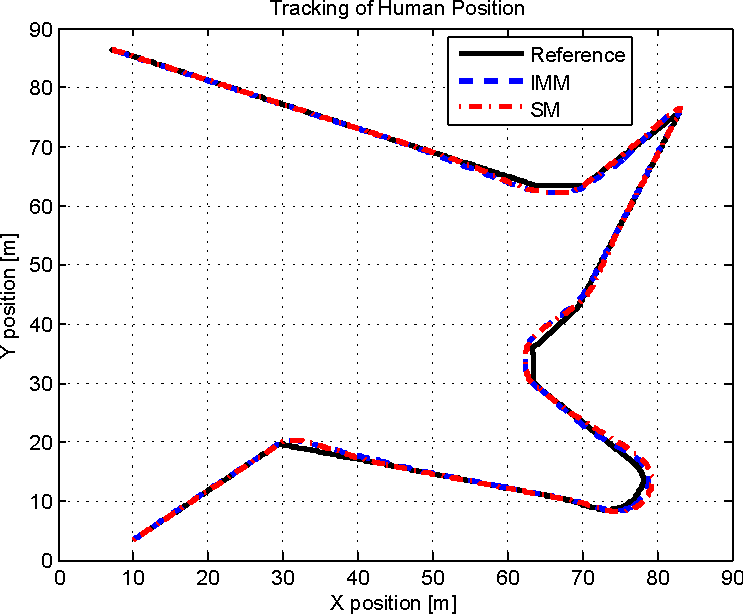
\includegraphics[width=0.38\textwidth]{figures/track_perform}
	%\caption{Comparison of tracking performance using the IMM-based and single-model approaches}
	%\label{fig:track_perform}
	%\end{figure}
	
	\begin{figure}
		\centering
		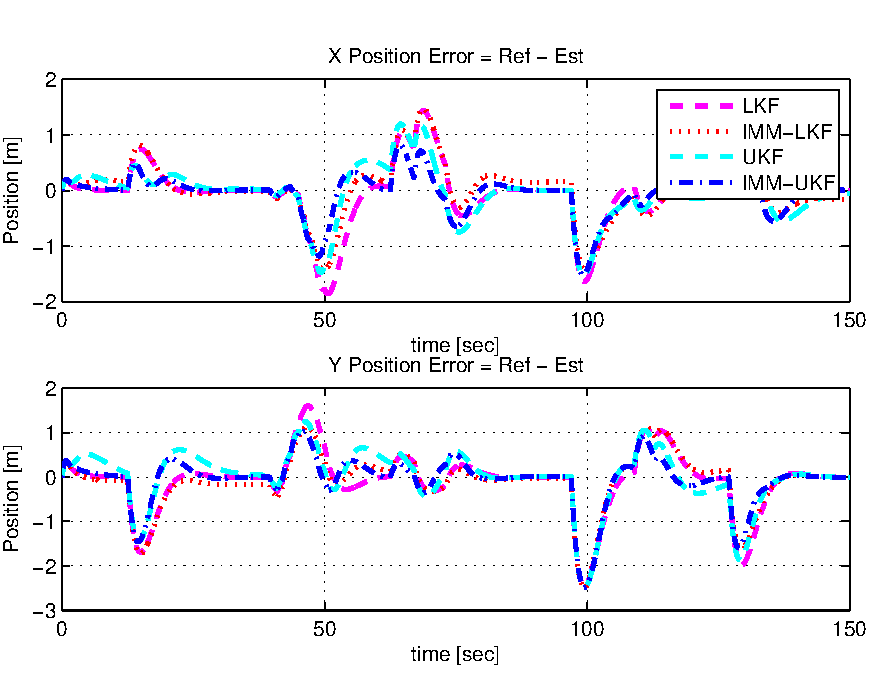
\includegraphics[width=0.4\textwidth]{figures/pos_error}
		\caption{Comparison of position estimation error with LKF, IMM-LKF, UKF and IMM-UKF}
		\label{fig:track_pos}
	\end{figure}
	
	\begin{figure}
		\centering
		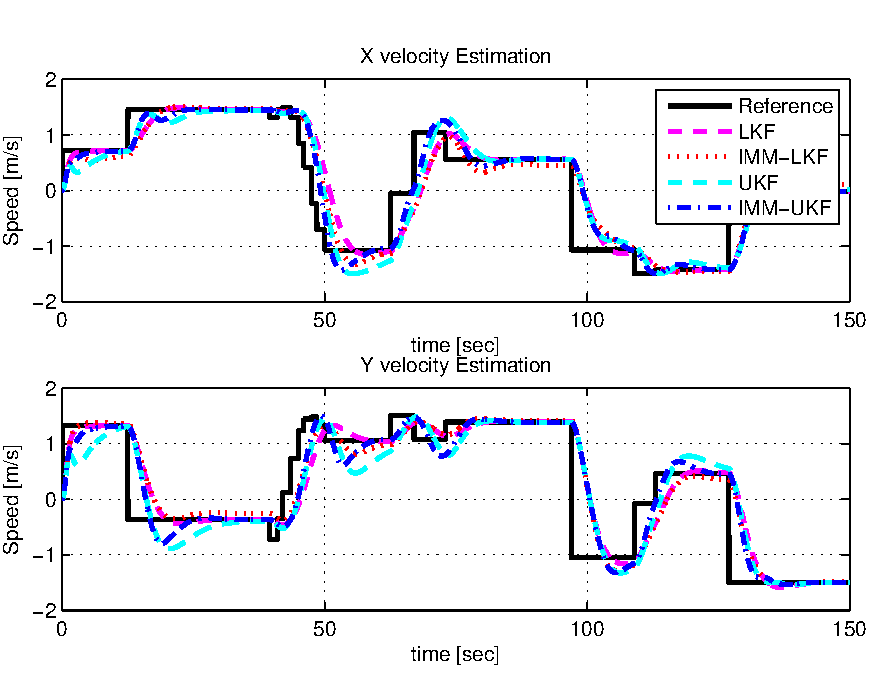
\includegraphics[width=0.4\textwidth]{figures/VelocityComp}
		\caption{Comparison of the estimated velocity using the IMM-based and the single-model approaches}
		\label{fig:track_v}
	\end{figure}
	
	\begin{figure}
		\centering
		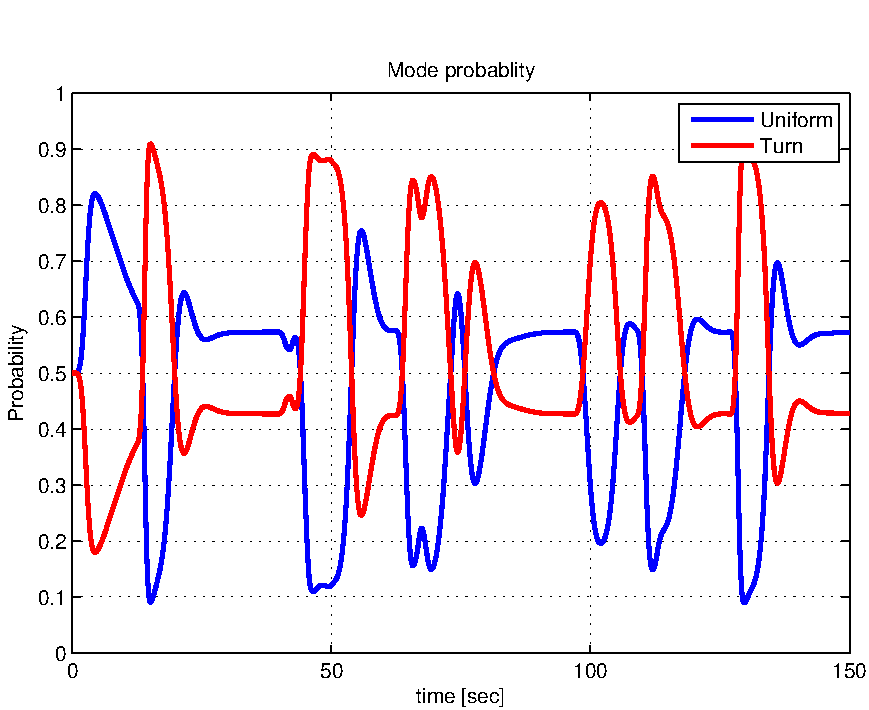
\includegraphics[width=0.38\textwidth]{figures/mode_prob}
		\caption{Model probabilities of two models in the IMM-UKF estimator}
		\label{fig:mode_prob}
	\end{figure}
	%\todonote{resize the legend in figure 3}
	\cref{fig:track_pos} shows the position estimation error on longitudinal and lateral directions using four different estimators: Linear Kalman Filter (LKF), IMM-LKF, UKF and IMM-UKF. 
	In the simulation, the same turn motion model in IMM-UKF is adopted for the system dynamics in UKF and the uniform motion model in IMM-LKF is also applied to the dynamic model in LKF.  
	There are two observations in this figure. First, the responses of the nonlinear estimators such as UKF and IMM-UKF are faster than the linear estimators. Second, the IMM-based approaches show better performance in accuracy than the single-model approaches.
	Besided, IMM-UKF achieves the fastest response and best accuracy compared to other methods, especially when the human turns around the circular obstacle at time $50$ and makes sharp turn after arriving at a destination at time $110$. 
	% Two methods achieves similar performance while the IMM estimator shows smaller estimation error at time $55$ and $103$, when the human turns around the circular obstacle and makes sharp turn after arriving at a destination, respectively.
	\cref{fig:track_v} compares the velocity estimation using four estimators.
	Overall, the nonlinear estimators (UKF and IMM-UKF) show faster response compared to the linear estimators (LKF and IMM-LKF), though they have overshoots due to the fast response. 
	It is worth noting that the overshoots of IMM-UKF are smaller than UKF while keeping the fast response at time $53$ and $118$ when the velocity changes abruptly.    
	% We can notice that, IMM estimator achieves faster tracking than the single-model approach when the velocity changes abruptly.
	This makes sense as the UKF-IMM estimator incorporates uniform motion model that can capture the sudden velocity changes.
	\cref{fig:mode_prob} shows the mode probabilities of the uniform motion model and turn motion model in IMM-UKF over time.
	When the human speed changes, the mode probability of the turn motion becomes higher than that of the uniform motion. 
	These changes illustrates the reason that IMM-based estimators achieve more accurate and faster estimation than the single-model estimator at the sharp turn and circular turn, thus demonstrating the necessity of applying IMM-UKF estimator for human tracking.
	
	\subsubsection{Human motion prediction}\label{subsubsec:motion_pred}
	To evaluate the IMM-based prediction approaches, the average prediction error over the prediction horizon is computed and compared with the single-model approaches. 
	At time $k$, the prediction error is defined as:
	\begin{equation}
		\Delta_p(k)=\frac{1}{N}\sum\limits_{i=1}^{N}||\tilde{p}^h(k+i|k)-p^h(k+i)||_2\label{eqn:pred_err}
	\end{equation}
	
	Different from the IMM-based prediction approaches that extrapolate the human position by a weighted sum of the predicted positions from each model, the single-model methods only utilize the uniform motion model for prediction.
	
	
	\begin{figure}
		\centering
		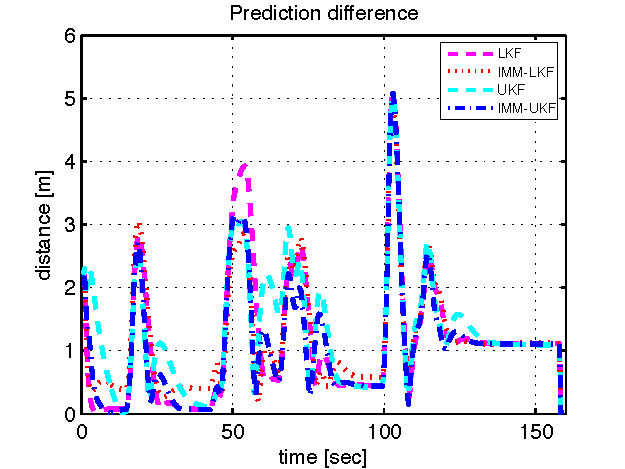
\includegraphics[width=0.42\textwidth]{figures/imm_vs_single}
		\caption{Comparison of prediction error between the IMM-based and single-model approaches}
		\label{fig:pred}
	\end{figure}
	% \begin{table} 
	% \centering
	% \begin{tabular}{|c|c|c|}
	% \hline
	% & mean & std\\ \hline
	% KF & 1.1435 & 1.0379\\ \hline
	% IMM-KF & 1.1927 & 0.8647\\ \hline
	% UKF & 1.2794 & 0.9104 \\ \hline
	% IMM-UKF & 1.0781 & 0.9094 \\ \hline
	% \end{tabular}
	% \caption{mean and standard deviation of prediction error}
	% \label{table:pre_err}
	% \end{table}
	
	\cref{fig:pred} shows the comparison of prediction error using two single-model approaches (LKF, UKF) and two IMM-based methods (IMM-LKF, IMM-UKF).
	It can be noticed that single-model approaches generate larger prediction error than IMM-based methods, especially when the human makes turns,  such as at time $50$.
	This makes sense as IMM-based method considers different dynamic models related to the human motion.
	% \cref{table:pre_err} lists the mean and standard deviation of the prediction error using these four methods.
	% It shows that the IMM-UKF achieves minimum mean error and the IMM-KF results in the smallest standard deviation.
	Based on the simulation results, IMM-UKF outperforms the other three methods for prediction.
	%For the times when the human moves in straight lines without changes in heading, the IMM-based method and the single-model approach achieves similar accuracy.
	%However, since we use a simple human behavior that the human keeps constant speed and moves in straight lines without changes in heading for a large portion of the trajectory, the single-model approach can achieve similar prediction performance as the IMM-based method.
	%However, since the human keeps constant speed and moves in straight lines without changes in heading for a large portion of the trajectory, the single-model approach can achieve similar prediction performance as the IMM-based method.
	
	\subsubsection{Robot motion planning}\label{subsubsec:motion_plan}
	\cref{fig:robot_accom} shows the trajectory of the companion robot that accompanies the target person moving in the field. The trajectory is generated by the proposed MPC motion planner and using the IMM-UKF for predicting human and moving obstacles' trajectories.
	The performance of the motion planning is evaluated using the criterion of safety and comfort.
	To be specific, the distance and speed differences between the robot and the human at each time step are measured, which are defined as:
	\begin{subequations}
		\begin{align}
			\Delta_d(k)&=||p^r(k)-p^h(k)||_2-d_s\label{eqn:err_d}\\
			\Delta_v(k)&=|v^r(k)-v^h(k)|\label{eqn:err_v}
		\end{align}
	\end{subequations}
	These quantities are illustrated as the blue line in \cref{fig:err_d,fig:err_v}.
	
	The performance of IMM-UKF predictor for robot motion planning is evaluated by comparing with two benchmark prediction strategies, while using the same MPC planner.
	The first benchmark method applies a single-model predictor (UKF predictor) to the coordinate turn motion model \todoQ{Dong-han, is this correct?} and predicts human motion.
	The second one does not predict human motion.
	Instead, the robot only utilize the human's current state for one-step motion planning.
	%We compare the MPC-based motion planning with a commonly used reactive motion planning method. %using \cref{eqn:err_d,eqn:err_v}.
	%With the reactive method, the robot uses one-step prediction of human position and heads for it while keeping the safe distance from the human and matching up with the human speed.
	%Both methods utilize the predicted human states from the IMM-UKF estimation and prediction methods.
	\begin{figure}
		\centering
		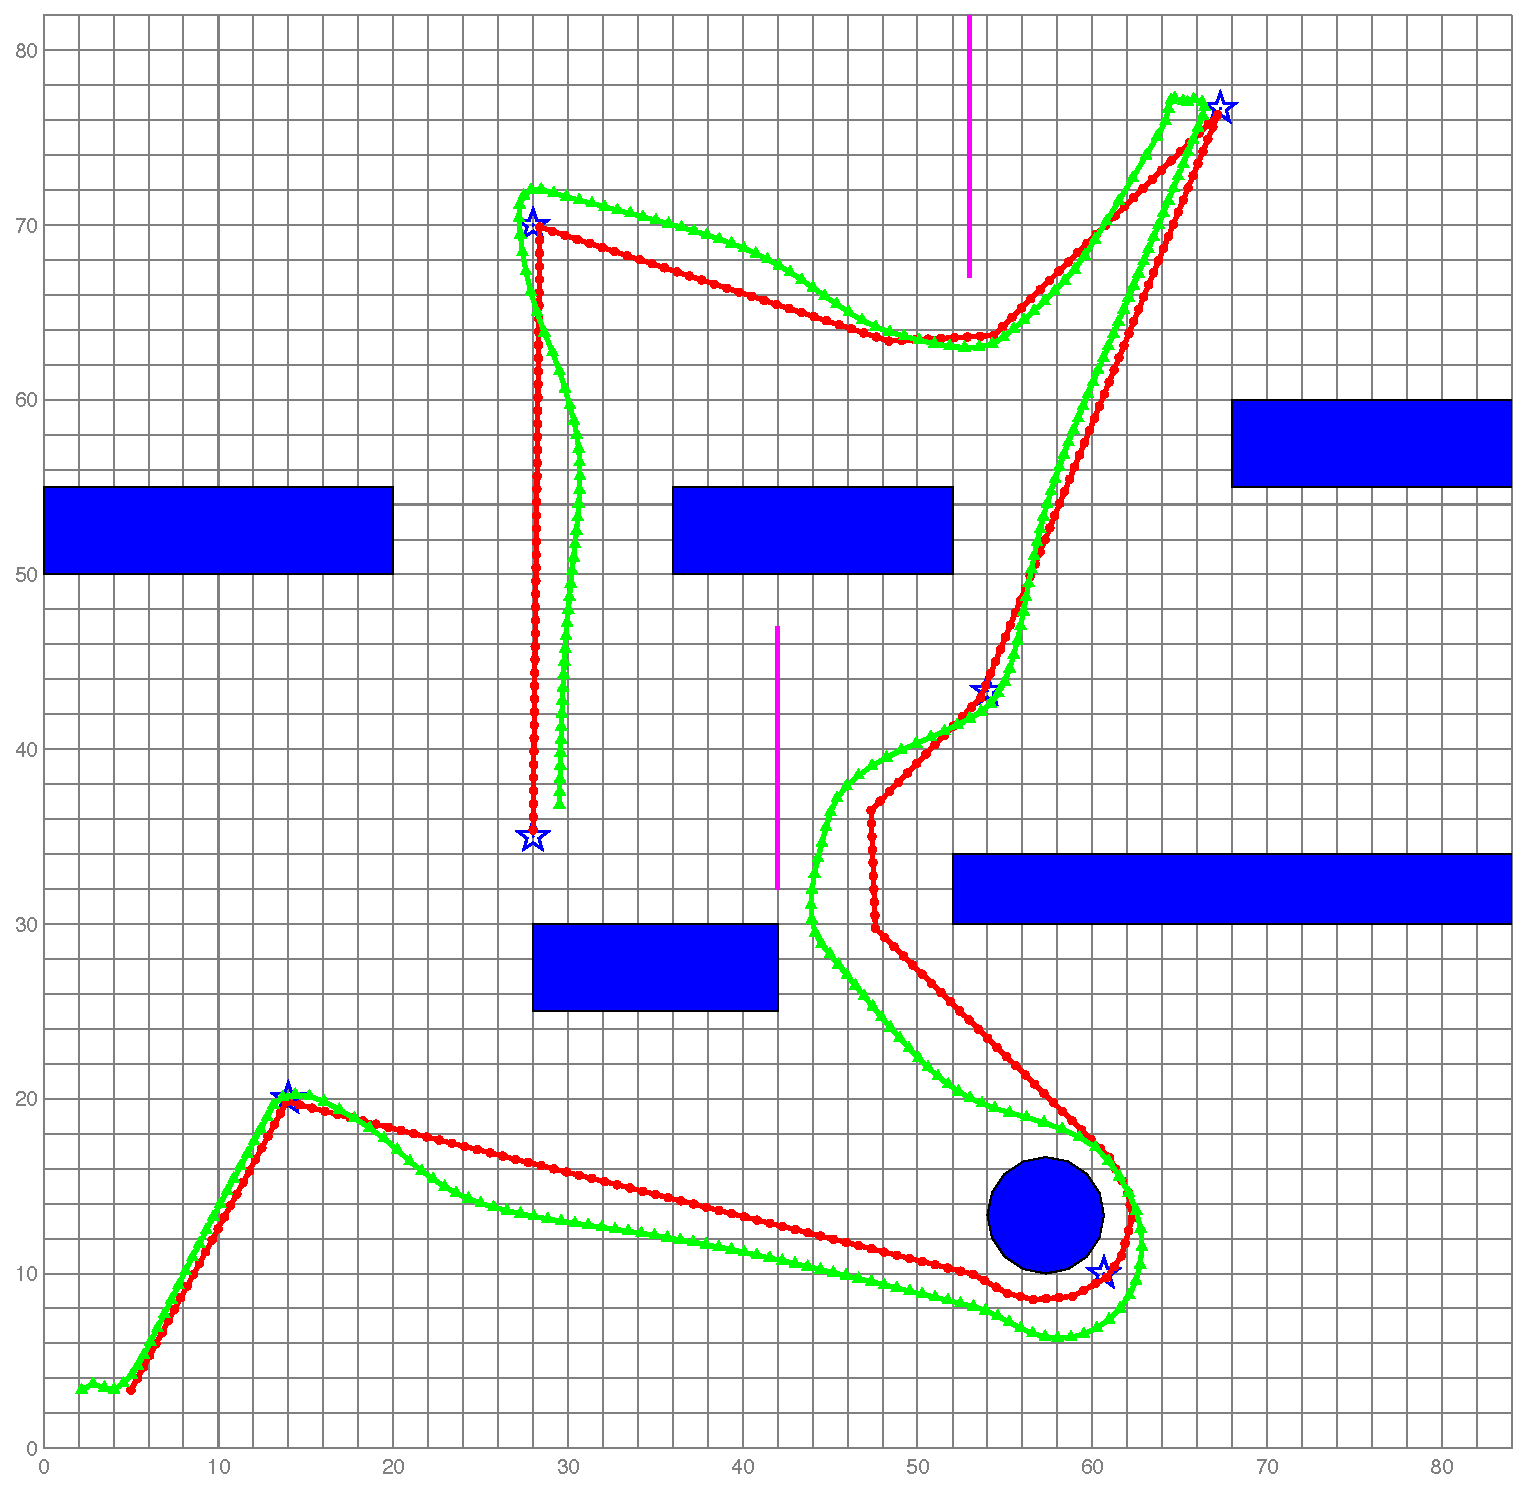
\includegraphics[width=0.37\textwidth]{figures/r_accomp.pdf}
		\caption{A screenshot of the simulation. The red line represents the human trajectory and the green on shows the companion robot's trajectory. For most of the time, the robot follows the human from behind\todohere{legend uses upper}}
		\label{fig:robot_accom}
	\end{figure}
	\begin{figure}
		\centering
		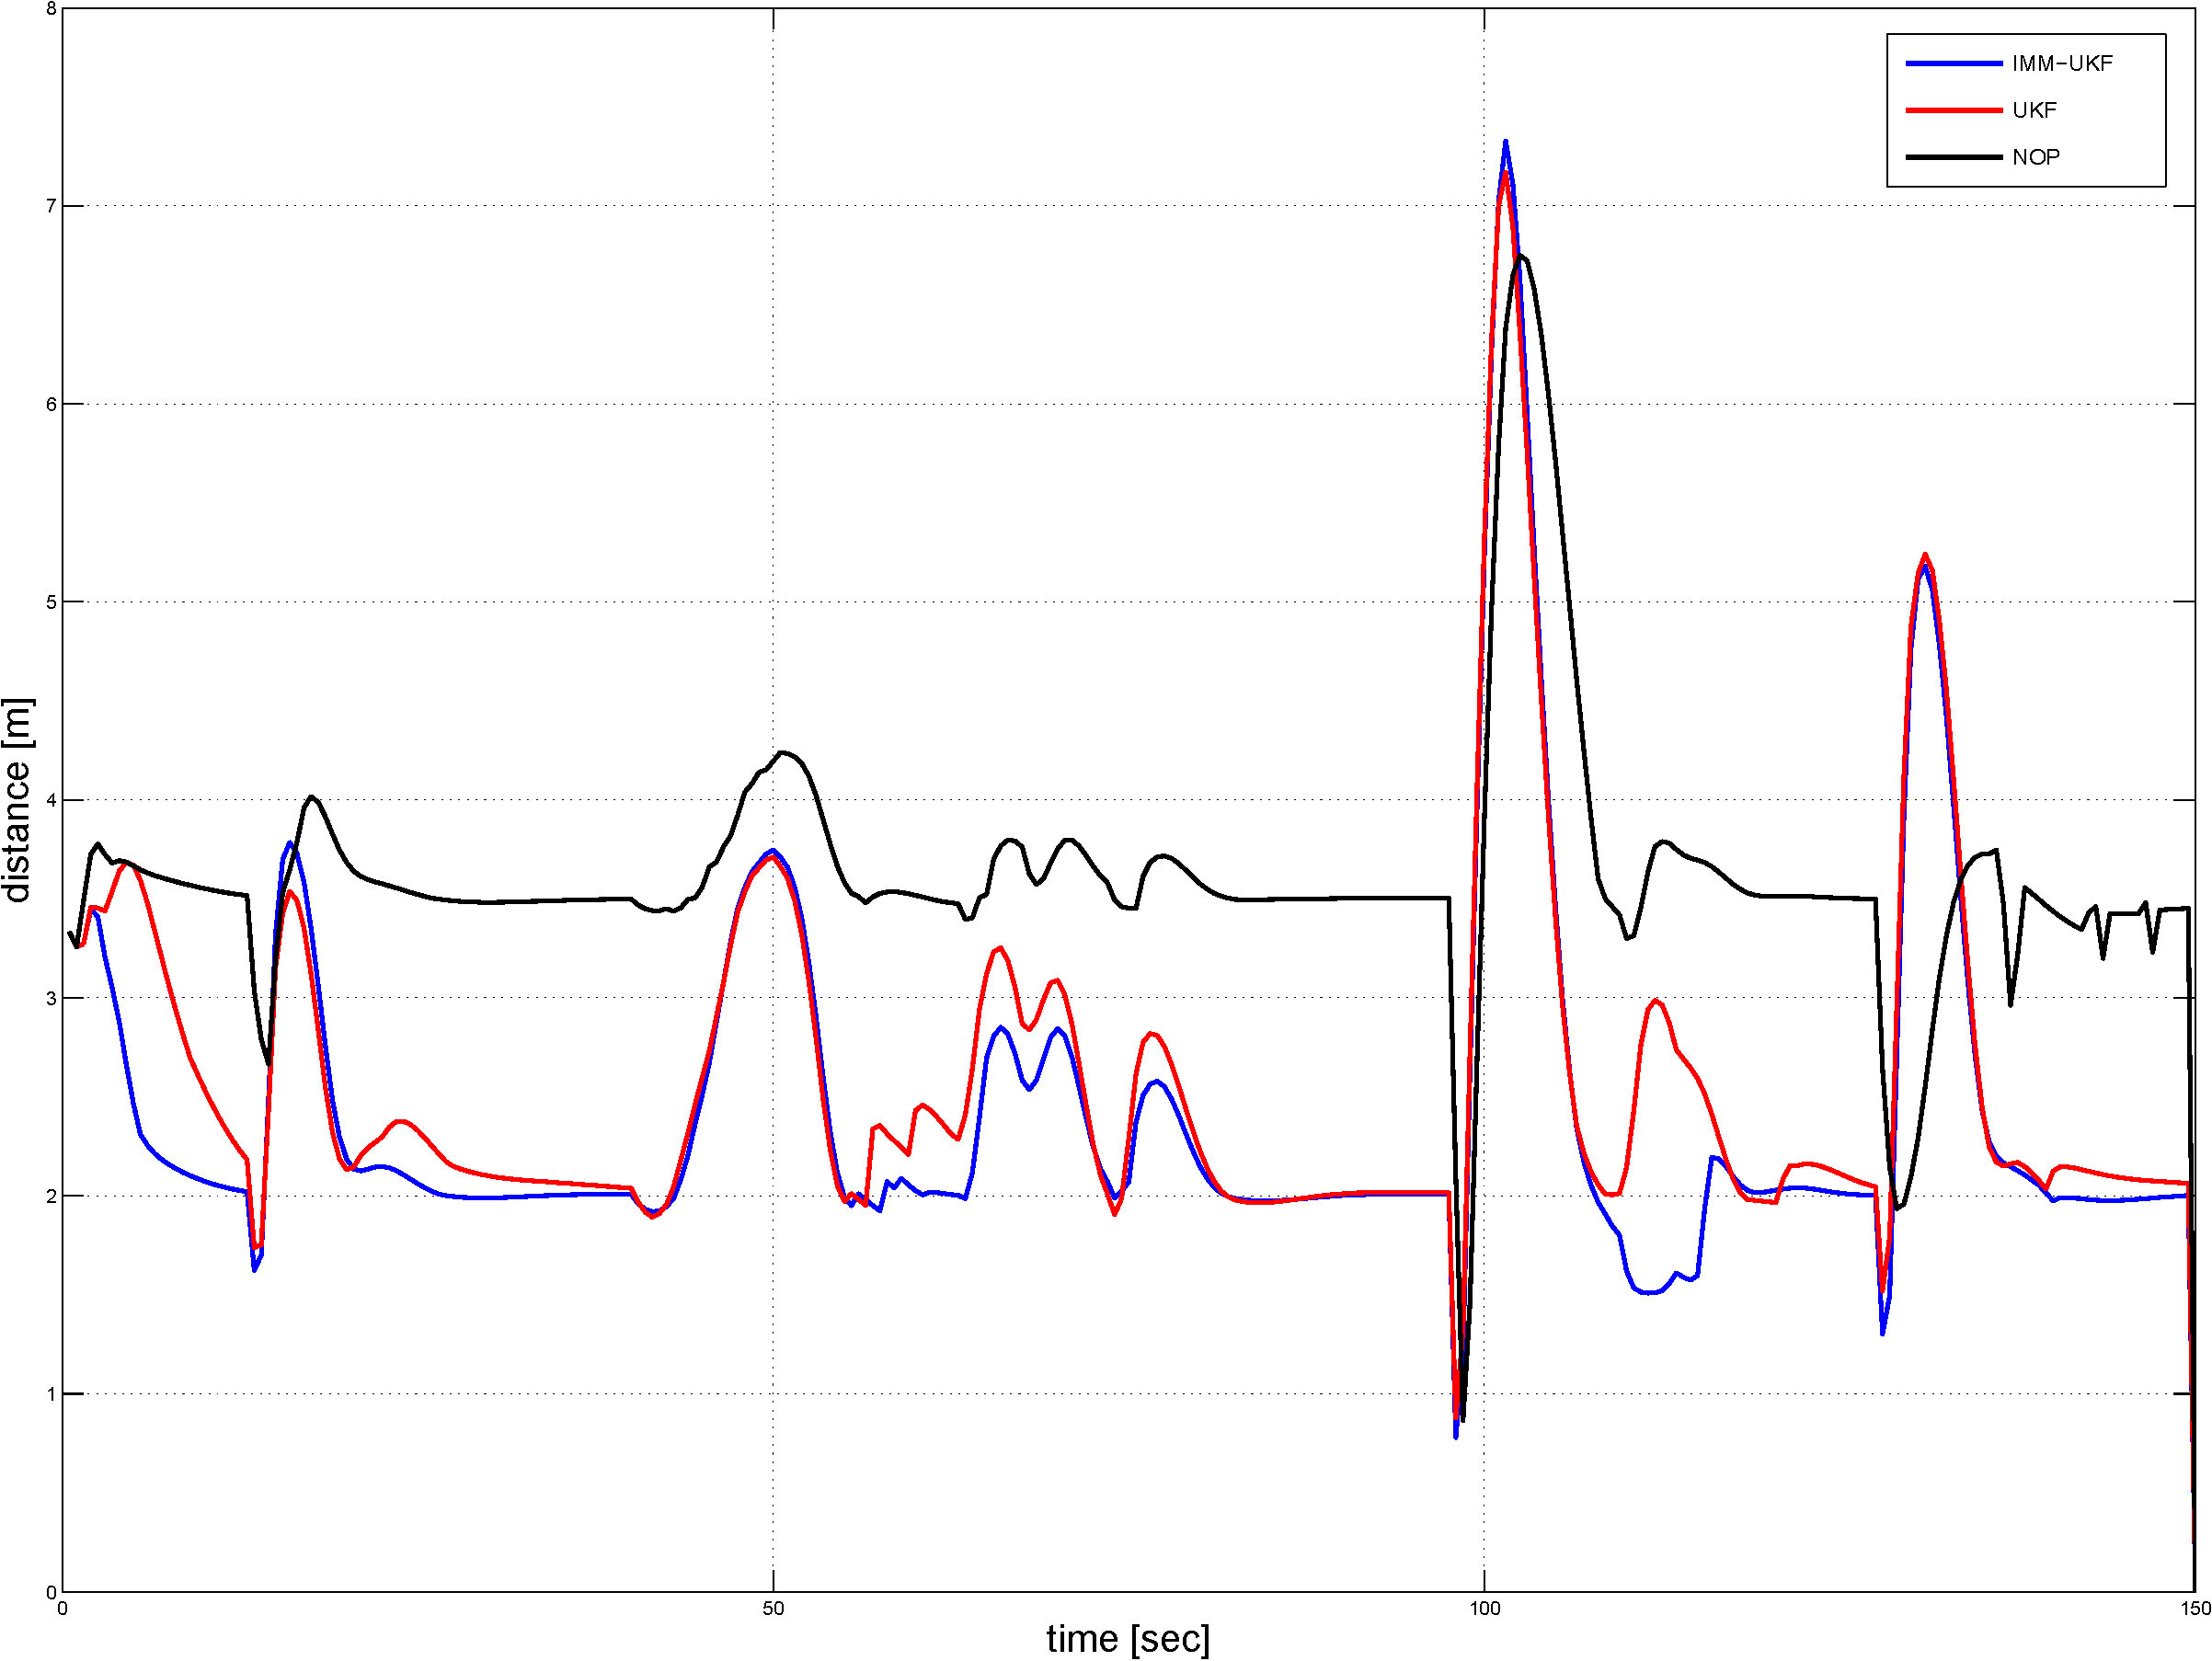
\includegraphics[width=0.37\textwidth]{figures/dis_diff.pdf}
		\caption{Comparison of distance (substracted by the safety distance) between the human and the robot using the MPC and the reactive methods}
		\label{fig:err_d}
	\end{figure}
	
	\begin{figure}
		\centering
		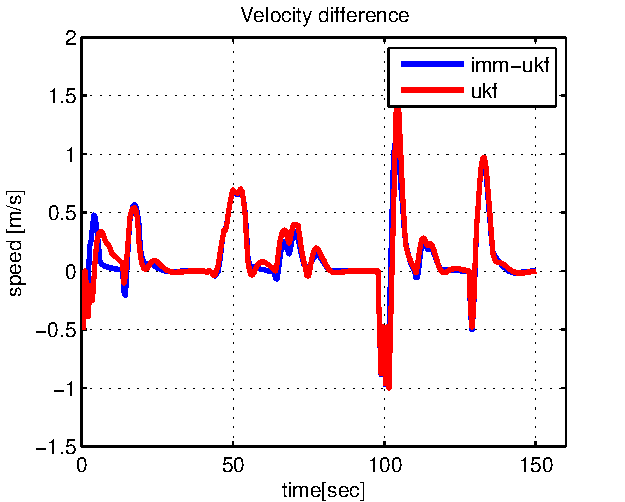
\includegraphics[width=0.37\textwidth]{figures/vel_diff.pdf}
		\caption{Comparison of velocity difference between the human and the robot using the MPC and the reactive methods}
		\label{fig:err_v}
	\end{figure}
	
	\begin{table}
		\caption{human-robot distance}
		\captionsetup{width=.5\textwidth}
		\centering
		\begin{tabular}{|c|c|c|c|}
			\hline
			Method & IMM-UKF & UKF & non-prediction\\
			\hline
			Ave & 1.4323 & 1.5890 & 2.6053\\
			\hline
			Std & 0.9367 & 0.9023 & 0.6428\\
			\hline
		\end{tabular}
		\label{table:distance}
	\end{table}
	
	\begin{table}
		\caption{speed difference}
		\captionsetup{width=.5\textwidth}
		\centering
		\begin{tabular}{|c|c|c|c|}
			\hline
			Method & IMM-UKF & UKF & non-prediction\\
			\hline
			Ave & 0.1018 & 0.1194 & 0.0189\\
			\hline
			Std & 0.2588 & 0.2510 & 0.2032\\
			\hline
		\end{tabular}
		\label{table:speed}
	\end{table}
	
	\cref{fig:err_d} compares the distances between the human and the robot using these threestrategies.
	Notice that the distances in the plot has been substracted by the safety distance $d_s$.
	Therefore, distance values less than zero at any time step are considered unsafe and thus undesirable.
	In addition, distance around $d_c-d_s$ is desired, as it implies that the robot keeps a comfortable distance $d_c$ from the human.
	It can be noticed that the MPC planner has ensured the safety of the accompanied human with each of the three prediction methods. 
	Additionally, by incorporating human motion prediction into the motion planning, the robot improves its companion performance from the non-prediction case.
	This can be demonstrated by \cref{table:distance} that the mean of human-robot distance using the prediction is much smaller than that without prediction.
	Additionally, the IMM-UKF predictor achieves better performance than the UKF-predictor in that the average distance is smaller but still within the comfort range using the former predictor than with the latter one.
	%On the contrary, the reactive method results in distances greater than $1$ for xxx\% of time while the smallest distance drops to $-xxx$ at time xxx.
	% 	The IMM-UKF method achieves xxx\% improvement on average distance, xxx\% on maximum distance and also minimum distance. 
	% 	In addition, the robot using IMM-UKF as the predictor can achieve less unsafe distance than the other two approaches. 
	% 	Such improvement is desirable for an accompanying robot as it keeps proper distance from the human and only moves within the unsafe distance for xxx long. 
	% 	Such unsafty is caused when the human makes sharp turns and the prediction deviates from the actual positions, which has been discussed in \cref{subsubsec:motion_est,subsubsec:motion_pred}.
	%Specifically, when the human makes a sharp turn at $103 s$, the MPC approach generates distance differences up to 8 while the reactive method results in almost 14.
	%% Due to the robot's limited angular velocity, the distance difference becomes large, with the peak values being $7.288$ for the MPC method at time $109.5s$ and $7.844$ for the reactive method at time $110.5$.
	%% The distance difference drops to $0.060$ at time 113 using the MPC method, showing that the robot accelerates to catch up with the human.
	%% This process can be seen in \cref{fig:err_v}.
	%% However, the reactive method maintains large distance between the human and the robot, with the minimum distance of 6.551, after time $109.5s$.
	%% This shows the benefits of using the MPC framework for motion planning compared to the reactive approach.
	%The differences mainly comes from the multiple-step prediction that the MPC method utilizes.
	%Due to the limited acceleration and angular velocity, the robot needs to predict several steps ahead in order to stay within the proper distance from the human.
	%The reactive method, however, only takes into account one-step prediction.
	%This myopic strategy renders the robot less capable to adjust its states for human's future positions.
	%Another benefit of using MPC method comes from its natural incorporation of various requirements by formulating them as the objective function and the constraints.
	%In contrast, designing a reactive method that considers different requirements becomes time-consuming and even infeasible when the complexity of requirements increases.
	%\cref{fig:err_v} compares the velocity differences between the human and the robot using these two methods.
	%It can be noticed that both approaches result in comparable velocity differences.
	
	The non-prediction method achieves smaller velocity difference than methods using predictors.
	This seems to imply that the non-prediction method is preferable for robot to similar pace as the human.
	However, such similarity using non-prediction method results in unsatisfactory following behavior, as shown in \cref{fig:err_d}.
	%     The benefits of including human motion prediction is also demonstrated by comparing the velocity differences, as shown in \cref{fig:err_v}.
	%     UKF and IMM-UKF predictor result in smaller differences than the non-prediction method.
	%     Moreover, the statistics shows smaller velocity difference using the IMM-UKF predictor.	
	In general, the simulation results show the superiority of using the multiple-model predictor (IMM-UKF predictor) for robot motion planning.
	% This makes sense as we explicitly requires the robot to match up with the human speed using the reactive method while in MPC method the velocity difference only composes one term in the objective function with a smaller weight than the distance term.
	% However, in spite of the small speed difference using the reactive method, the resultant large human-robot distance, as shown in \cref{fig:err_d}, renders such closeness on speed less attractive.
	% In fact, the proper distance between the human and the robot composes the core part of a human-accompanying robot.
	
	\section{CONCLUSION}\label{sec:conclusion}
	We have developed a model predictve control (MPC)-based motion planning approach for human-companion robots to accompany a target person in a socially desirable manner, which considers the safety and comfort of the behavior.
	Such companion robot can be useful for search and rescue scenarios by carrying apparatus, exploring dangerous areas and detecting survivors.
	The IMM-UKF approach that incorporates the uniform motion model and the coordinated turn motion models is developed for human position estimation and prediction.
	Such multiple-model approach captures different motion patterns, thus improving the estimation and prediction accuracy than other single-model approaches.
	Based on the predicted human positions, the model predictive control (MPC) approach is formulated for planning socially desirable motion trajectory.
	The estimation and prediction accuracy using IMM-UKF is compared with IMM-LKF and two single-model methods (LFK and UKF).
	Comparison results show superior accuracy and response in estimation and prediction using IMM-UKF approach, especially when the human makes circular motion or sharp turns.
	Moreover, the MPC planner using IMM-UKF predictor, UKF predictor and no predictor are compared.
	The IMM-UKF predictor improves the robot motion behavior that keeps human-robot distances around the comfort distance and similar velocity.
	%	The MPC motion planning approach is compared with a reactive method and shows that the MPC method achieves better performance in generating smaller human-robot distance while similar performance in the velocity difference.
	% The reactive policy achieves smaller velocity differences than the MPC method.
	% However, this becomes less attractive as the resultant human-robot distance becomes very large.
	
	In the future work, we plan to investigate other motion prediction methods, such as the autoregressive–moving-average method, to compare with IMM-UKF method.
	Besides,  enabling the robot to learn human motion model in real time is an attractive topic and may provide more accurate human motion prediction and results in better human-companion behaviors.
	
	%%%%%%%%%%%%%%%%%%%%%%%%%%%%%%%%%%%%%%%%%%%%%%%%%%%%%%%%%%%%%%%%%%%%%%%%%%%%%%%%
	
	%\appendix
	\section{APPENDIX}
	\subsection{IMM-LKF Predictor}
	Similar to IMM-UKF, IMM-LKF works with two dynamic models: one is the uniform motion model; the other is the coordinated turn motion model. If the turn rate is a known constant in the coordinated turn motion model in \cref{eqn:h_c_dyn}, the human estimation procedure can be modeled with the discrete time linear state space system as follows:
	\begin{subequations}
		\begin{align}
			x^h(k+1) = Ax^h(k)+B_ww(k)\label{eqn:h_dyn}\\
			y^h(k)=Cx^h(k)+v(k)\label{eqn:observation}
		\end{align}
	\end{subequations}
	where $x^h(k)$ and $y^h(k)$ represent the human motion state and the observation, respectively, at the time step $k$; $w(k)$ and $v(k)$ represent process noise and measurement noise, respectively.
	$x^h(k)$ consists of four elements: $p^h_1,v^h_1,p^h_2,v^h_2$, where $p^h_1,p^h_2$ denote the longitudinal and lateral position of the human and $v^h_1,v^h_2$ the corresponding velocity.
	We use two Linear Kalman Filters in the IMM for human tracking, each corresponding to a different dynamics model: the uniform motion model and the turn motion model.
	Two models differ in the $A$ matrix and $w$ in \cref{eqn:h_dyn} while sharing the same $B_w$.
	In particular, we define the matrices as follows:
	\begin{subequations}
		\begin{align}
			A_U&=\left[
			\begin{array}{cccc}
				1& T& 0& 0\\
				0& 1& 0& 0\\
				0& 0& 1& T\\
				0& 0& 0& 1
			\end{array}\right],\label{eqn:A_U}\\
			A_T&=\left[
			\begin{array}{cccc}
				1& \frac{\sin(\omega T)}{\omega}& 0& \frac{1-\cos(\omega T)}{\omega}\\
				0& \cos(\omega T)& 0& -\sin(\omega T)\\
				0& \frac{1-\cos(\omega T)}{\omega}& 1& \frac{\sin(\omega T)}{\omega}\\
				0& \sin(\omega T)& 0& \cos(\omega T)
			\end{array}\right],\label{eqn:A_T}\\
			B_w&=\left[
			\begin{array}{cccc}
				\frac{T^2}{2}& T& 0& 0\\
				0& 0& \frac{T^2}{2}& T
			\end{array}\right],\label{eqn:B_w}\\
			w_U&\sim\mathcal{N}(0,Q_U)\; w_T\sim\mathcal{N}(0,Q_T)\label{eqn:pro_noise}
		\end{align}
	\end{subequations}
	where $A_U$ and $A_T$ stand for the $A$ matrices of the uniform motion model and turn motion model, respectively; $w_U$ and $w_T$ denote the process noise of the uniform motion model and turn motion model, respectively; $T$ represents the sampling time; $\omega$ represents the constant turn rate.
	
	We assume that only the human position can be measured.
	Therefore, the parameters in observation model \cref{eqn:observation} can be defined as:
	\begin{subequations}
		\begin{align}
			C&=\left[
			\begin{array}{cccc}
				1& 0& 0& 0\\
				0& 0& 1& 0
			\end{array}\right],\label{eqn:C}\\
			v&\sim\mathcal{N}(0,V)\label{eqn:meas_noise}
		\end{align}
	\end{subequations}
	Above linear state space models are used in LKF and IMM-LKF in this paper.
	Moreover, we set the turn rate $\omega$ to be $0.1$ rad/s as a known constant, in the turn motion model in IMM-LKF. 
	
	\subsection{Approximating Static Obstacles}
	Static rectangular obstacles are approximated and analytically represented as ellipses, as shown in \cref{fig:ellipse_approx}.
	Let $l$ and $m$ be the length and width of a rectangular obstacle centered at the origin.
	Let \cref{eqn:ellipse} represent the ellipse that encloses the obstacle in the way that the four vertices of the rectangle lie on the boundary of the ellipse.
	\begin{equation*}\label{eqn:ellipse}
		\frac{x^2}{a^2}+\frac{y^2}{b^2}=1
	\end{equation*}
	In addition, assume that the rectangle and ellipse have the same aspect ratio, which means $\frac{l}{m}=\frac{a}{b}$, then $a=\frac{l}{\sqrt{2}}$ and $b=\frac{m}{\sqrt{2}}$.
	
	
	
	\addtolength{\textheight}{-12cm}   % This command serves to balance the column lengths
	% on the last page of the document manually. It shortens
	% the textheight of the last page by a suitable amount.
	% This command does not take effect until the next page
	% so it should come on the page before the last. Make
	% sure that you do not shorten the textheight too much.
	
	
	%%%%%%%%%%%%%%%%%%%%%%%%%%%%%%%%%%%%%%%%%%%%%%%%%%%%%%%%%%%%%%%%%%%%%%%%%%%%%%%%
	
	\bibliographystyle{ieeetr}
	\bibliography{references}
\end{document}